\documentclass[]{article}
\usepackage{lmodern}
\usepackage{amssymb,amsmath}
\usepackage{ifxetex,ifluatex}
\usepackage{fixltx2e} % provides \textsubscript
\ifnum 0\ifxetex 1\fi\ifluatex 1\fi=0 % if pdftex
  \usepackage[T1]{fontenc}
  \usepackage[utf8]{inputenc}
\else % if luatex or xelatex
  \ifxetex
    \usepackage{mathspec}
  \else
    \usepackage{fontspec}
  \fi
  \defaultfontfeatures{Ligatures=TeX,Scale=MatchLowercase}
\fi
% use upquote if available, for straight quotes in verbatim environments
\IfFileExists{upquote.sty}{\usepackage{upquote}}{}
% use microtype if available
\IfFileExists{microtype.sty}{%
\usepackage{microtype}
\UseMicrotypeSet[protrusion]{basicmath} % disable protrusion for tt fonts
}{}
\usepackage[margin=1in]{geometry}
\usepackage{hyperref}
\hypersetup{unicode=true,
            pdftitle={A guided tour in targeted learning territory},
            pdfauthor={David Benkeser, Antoine Chambaz, Nima Hejazi},
            pdfborder={0 0 0},
            breaklinks=true}
\urlstyle{same}  % don't use monospace font for urls
\usepackage{color}
\usepackage{fancyvrb}
\newcommand{\VerbBar}{|}
\newcommand{\VERB}{\Verb[commandchars=\\\{\}]}
\DefineVerbatimEnvironment{Highlighting}{Verbatim}{commandchars=\\\{\}}
% Add ',fontsize=\small' for more characters per line
\usepackage{framed}
\definecolor{shadecolor}{RGB}{248,248,248}
\newenvironment{Shaded}{\begin{snugshade}}{\end{snugshade}}
\newcommand{\AlertTok}[1]{\textcolor[rgb]{0.94,0.16,0.16}{#1}}
\newcommand{\AnnotationTok}[1]{\textcolor[rgb]{0.56,0.35,0.01}{\textbf{\textit{#1}}}}
\newcommand{\AttributeTok}[1]{\textcolor[rgb]{0.77,0.63,0.00}{#1}}
\newcommand{\BaseNTok}[1]{\textcolor[rgb]{0.00,0.00,0.81}{#1}}
\newcommand{\BuiltInTok}[1]{#1}
\newcommand{\CharTok}[1]{\textcolor[rgb]{0.31,0.60,0.02}{#1}}
\newcommand{\CommentTok}[1]{\textcolor[rgb]{0.56,0.35,0.01}{\textit{#1}}}
\newcommand{\CommentVarTok}[1]{\textcolor[rgb]{0.56,0.35,0.01}{\textbf{\textit{#1}}}}
\newcommand{\ConstantTok}[1]{\textcolor[rgb]{0.00,0.00,0.00}{#1}}
\newcommand{\ControlFlowTok}[1]{\textcolor[rgb]{0.13,0.29,0.53}{\textbf{#1}}}
\newcommand{\DataTypeTok}[1]{\textcolor[rgb]{0.13,0.29,0.53}{#1}}
\newcommand{\DecValTok}[1]{\textcolor[rgb]{0.00,0.00,0.81}{#1}}
\newcommand{\DocumentationTok}[1]{\textcolor[rgb]{0.56,0.35,0.01}{\textbf{\textit{#1}}}}
\newcommand{\ErrorTok}[1]{\textcolor[rgb]{0.64,0.00,0.00}{\textbf{#1}}}
\newcommand{\ExtensionTok}[1]{#1}
\newcommand{\FloatTok}[1]{\textcolor[rgb]{0.00,0.00,0.81}{#1}}
\newcommand{\FunctionTok}[1]{\textcolor[rgb]{0.00,0.00,0.00}{#1}}
\newcommand{\ImportTok}[1]{#1}
\newcommand{\InformationTok}[1]{\textcolor[rgb]{0.56,0.35,0.01}{\textbf{\textit{#1}}}}
\newcommand{\KeywordTok}[1]{\textcolor[rgb]{0.13,0.29,0.53}{\textbf{#1}}}
\newcommand{\NormalTok}[1]{#1}
\newcommand{\OperatorTok}[1]{\textcolor[rgb]{0.81,0.36,0.00}{\textbf{#1}}}
\newcommand{\OtherTok}[1]{\textcolor[rgb]{0.56,0.35,0.01}{#1}}
\newcommand{\PreprocessorTok}[1]{\textcolor[rgb]{0.56,0.35,0.01}{\textit{#1}}}
\newcommand{\RegionMarkerTok}[1]{#1}
\newcommand{\SpecialCharTok}[1]{\textcolor[rgb]{0.00,0.00,0.00}{#1}}
\newcommand{\SpecialStringTok}[1]{\textcolor[rgb]{0.31,0.60,0.02}{#1}}
\newcommand{\StringTok}[1]{\textcolor[rgb]{0.31,0.60,0.02}{#1}}
\newcommand{\VariableTok}[1]{\textcolor[rgb]{0.00,0.00,0.00}{#1}}
\newcommand{\VerbatimStringTok}[1]{\textcolor[rgb]{0.31,0.60,0.02}{#1}}
\newcommand{\WarningTok}[1]{\textcolor[rgb]{0.56,0.35,0.01}{\textbf{\textit{#1}}}}
\usepackage{longtable,booktabs}
\usepackage{graphicx,grffile}
\makeatletter
\def\maxwidth{\ifdim\Gin@nat@width>\linewidth\linewidth\else\Gin@nat@width\fi}
\def\maxheight{\ifdim\Gin@nat@height>\textheight\textheight\else\Gin@nat@height\fi}
\makeatother
% Scale images if necessary, so that they will not overflow the page
% margins by default, and it is still possible to overwrite the defaults
% using explicit options in \includegraphics[width, height, ...]{}
\setkeys{Gin}{width=\maxwidth,height=\maxheight,keepaspectratio}
\IfFileExists{parskip.sty}{%
\usepackage{parskip}
}{% else
\setlength{\parindent}{0pt}
\setlength{\parskip}{6pt plus 2pt minus 1pt}
}
\setlength{\emergencystretch}{3em}  % prevent overfull lines
\providecommand{\tightlist}{%
  \setlength{\itemsep}{0pt}\setlength{\parskip}{0pt}}
\setcounter{secnumdepth}{5}
% Redefines (sub)paragraphs to behave more like sections
\ifx\paragraph\undefined\else
\let\oldparagraph\paragraph
\renewcommand{\paragraph}[1]{\oldparagraph{#1}\mbox{}}
\fi
\ifx\subparagraph\undefined\else
\let\oldsubparagraph\subparagraph
\renewcommand{\subparagraph}[1]{\oldsubparagraph{#1}\mbox{}}
\fi

%%% Use protect on footnotes to avoid problems with footnotes in titles
\let\rmarkdownfootnote\footnote%
\def\footnote{\protect\rmarkdownfootnote}

%%% Change title format to be more compact
\usepackage{titling}

% Create subtitle command for use in maketitle
\newcommand{\subtitle}[1]{
  \posttitle{
    \begin{center}\large#1\end{center}
    }
}

\setlength{\droptitle}{-2em}

  \title{A guided tour in targeted learning territory}
    \pretitle{\vspace{\droptitle}\centering\huge}
  \posttitle{\par}
    \author{David Benkeser, Antoine Chambaz, Nima Hejazi}
    \preauthor{\centering\large\emph}
  \postauthor{\par}
      \predate{\centering\large\emph}
  \postdate{\par}
    \date{08/20/2018}

\usepackage{amsmath,interval,amssymb,xcolor,manfnt,tikz}

\makeatletter
\renewcommand\subsection{\@startsection{subsection}{3}{\z@}%
                                     {-3.25ex\@plus -1ex \@minus -.2ex}%
                                     {-1.5ex \@plus .2ex}%
                                     {\normalfont\normalsize\bfseries}}
\makeatother
\addtolength{\parskip}{.5\baselineskip}
\renewcommand*{\thefootnote}{\fnsymbol{footnote}}

\DeclareMathOperator{\Dirac}{Dirac}
\DeclareMathOperator{\expit}{expit}
\DeclareMathOperator{\logit}{logit}
\DeclareMathOperator{\Rem}{Rem}
\DeclareMathOperator{\Var}{Var}

\newsavebox\gearbox
\newcommand{\gearmacro}[5]{%
  % #1 number of teeths
  % #2 radius intern
  % #3 radius extern
  % #4 angle from start to end of the first arc
  % #5 angle to decale the second arc from the first 
  \foreach \i in {1,...,#1} {%
    [rotate=(\i-1)*360/#1]  (0:#2)  arc (0:#4:#2) {[rounded corners=1.5pt]
      -- (#4+#5:#3)  arc (#4+#5:360/#1-#5:#3)} --  (360/#1:#2)
  }}  
\newcommand{\makegear}{\begin{tikzpicture}
    \fill[gray] (0,0) circle (2cm);
    \draw[thick,rotate=12,fill=gray] \gearmacro{8}{2}{2.4}{20}{2};
    \draw[thick,fill=white] (0cm,0cm) circle(1.35cm);
  \end{tikzpicture}}
\sbox\gearbox{\resizebox{!}{2em}{\makegear}}
\newcommand{\gear}{\usebox{\gearbox}\;}

\newcommand{\bbO}{\mathbb{O}}
\newcommand{\bbP}{\mathbb{P}}
\newcommand{\bbR}{\mathbb{R}}
\newcommand{\calF}{\mathcal{F}}
\newcommand{\calM}{\mathcal{M}}
\newcommand{\calO}{\mathcal{O}}
\newcommand{\Exp}{\textrm{E}}
\newcommand{\Gbar}{\bar{G}}
\newcommand{\one}{\textbf{1}}
\newcommand{\Psihat}{\widehat{\Psi}}
\newcommand{\Qbar}{\bar{Q}}
\newcommand{\tcg}[1]{\textcolor{olive}{#1}}

\allowdisplaybreaks

%%% Local Variables:
%%% mode: latex
%%% TeX-master: t
%%% End:

\usepackage{amsthm}
\newtheorem{theorem}{Theorem}[section]
\newtheorem{lemma}{Lemma}[section]
\theoremstyle{definition}
\newtheorem{definition}{Definition}[section]
\newtheorem{corollary}{Corollary}[section]
\newtheorem{proposition}{Proposition}[section]
\theoremstyle{definition}
\newtheorem{example}{Example}[section]
\theoremstyle{definition}
\newtheorem{exercise}{Exercise}[section]
\theoremstyle{remark}
\newtheorem*{remark}{Remark}
\newtheorem*{solution}{Solution}
\begin{document}
\maketitle

{
\setcounter{tocdepth}{2}
\tableofcontents
}
\section{Introduction}

\tcg{This is a very first draft  of our article. The current *tentative* title
  is "A guided tour in targeted learning territory".}

\tcg{Explain our objectives and how we will meet them. Explain that the symbol
\textdbend indicates more delicate material.}

\tcg{Use sectioning a lot to ease cross-referencing.}

\tcg{Do we include  exercises? I propose we do, and  to flag the corresponding
subsections with symbol $\gear$.}

\begin{Shaded}
\begin{Highlighting}[]
\KeywordTok{set.seed}\NormalTok{(}\DecValTok{54321}\NormalTok{) ## because reproducibility matters...}
\KeywordTok{suppressMessages}\NormalTok{(}\KeywordTok{library}\NormalTok{(R.utils)) ## make sure it is installed}
\KeywordTok{suppressMessages}\NormalTok{(}\KeywordTok{library}\NormalTok{(tidyverse)) ## make sure it is installed}
\KeywordTok{suppressMessages}\NormalTok{(}\KeywordTok{library}\NormalTok{(caret)) ## make sure it is installed}
\NormalTok{expit <-}\StringTok{ }\NormalTok{plogis}
\NormalTok{logit <-}\StringTok{ }\NormalTok{qlogis}
\end{Highlighting}
\end{Shaded}

Function \texttt{expit} implements the link function
\(\expit : \bbR \to ]0,1[\) given by
\(\expit(x) \equiv (1 + e^{-x})^{-1}\). Function \texttt{logit}
implements its inverse function \(\logit : ]0,1[ \to \bbR\) given by
\(\logit(p) \equiv \log [p/(1-p)]\).

\section{A simulation study}
\label{sec:simulation:study}

\tcg{blabla}

\subsection{Reproducible experiment as a law.}
\label{subsec:as:a:law}

We are interested in a reproducible experiment. The generic summary of
how one realization of the experiment unfolds, our observation, is
called \(O\). We view \(O\) as a random variable drawn from what we call
the law \(P_{0}\) of the experiment. The law \(P_{0}\) is viewed as an
element of what we call the model. Denoted by \(\calM\), the model is
the collection of \textit{all} laws from which \(O\) can be drawn and
that meet some constraints. The constraints translate the knowledge we
have about the experiment. The more we know about the experiment, the
smaller is \(\calM\). In all our examples, model \(\calM\) will put very
few restrictions on the candidate laws.

Consider the following chunk of code:

\begin{Shaded}
\begin{Highlighting}[]
\NormalTok{draw_from_experiment <-}\StringTok{ }\ControlFlowTok{function}\NormalTok{(n, }\DataTypeTok{ideal =} \OtherTok{FALSE}\NormalTok{) \{}
\NormalTok{  ## preliminary}
\NormalTok{  n <-}\StringTok{ }\NormalTok{Arguments}\OperatorTok{$}\KeywordTok{getInteger}\NormalTok{(n, }\KeywordTok{c}\NormalTok{(}\DecValTok{1}\NormalTok{, }\OtherTok{Inf}\NormalTok{))}
\NormalTok{  ideal <-}\StringTok{ }\NormalTok{Arguments}\OperatorTok{$}\KeywordTok{getLogical}\NormalTok{(ideal)}
\NormalTok{  ## ## 'Gbar' and 'Qbar' factors}
\NormalTok{  Gbar <-}\StringTok{ }\ControlFlowTok{function}\NormalTok{(W) \{}
    \KeywordTok{expit}\NormalTok{(}\DecValTok{1} \OperatorTok{+}\StringTok{ }\DecValTok{2} \OperatorTok{*}\StringTok{ }\NormalTok{W }\OperatorTok{-}\StringTok{ }\DecValTok{4} \OperatorTok{*}\StringTok{ }\KeywordTok{sqrt}\NormalTok{(}\KeywordTok{abs}\NormalTok{((W }\OperatorTok{-}\StringTok{ }\DecValTok{5}\OperatorTok{/}\DecValTok{12}\NormalTok{))))}
\NormalTok{  \}}
\NormalTok{  Qbar <-}\StringTok{ }\ControlFlowTok{function}\NormalTok{(AW) \{}
\NormalTok{    A <-}\StringTok{ }\NormalTok{AW[, }\DecValTok{1}\NormalTok{]}
\NormalTok{    W <-}\StringTok{ }\NormalTok{AW[, }\DecValTok{2}\NormalTok{]}
\NormalTok{    ## A * (cos((1 + W) * pi / 4) + (1/3 <= W & W <= 1/2) / 5) +}
\NormalTok{    ##  (1 - A) * (sin(4 * W^2 * pi) / 4 + 1/2)}
\NormalTok{    A }\OperatorTok{*}\StringTok{ }\NormalTok{(}\KeywordTok{cos}\NormalTok{((}\OperatorTok{-}\DecValTok{1}\OperatorTok{/}\DecValTok{2} \OperatorTok{+}\StringTok{ }\NormalTok{W) }\OperatorTok{*}\StringTok{ }\NormalTok{pi) }\OperatorTok{*}\StringTok{ }\DecValTok{2}\OperatorTok{/}\DecValTok{5} \OperatorTok{+}\StringTok{ }\DecValTok{1}\OperatorTok{/}\DecValTok{5} \OperatorTok{+}\StringTok{ }\NormalTok{(}\DecValTok{1}\OperatorTok{/}\DecValTok{3} \OperatorTok{<=}\StringTok{ }\NormalTok{W }\OperatorTok{&}\StringTok{ }\NormalTok{W }\OperatorTok{<=}\StringTok{ }\DecValTok{1}\OperatorTok{/}\DecValTok{2}\NormalTok{) }\OperatorTok{/}\StringTok{ }\DecValTok{5} \OperatorTok{+}
\StringTok{         }\NormalTok{(W }\OperatorTok{>=}\StringTok{ }\DecValTok{3}\OperatorTok{/}\DecValTok{4}\NormalTok{) }\OperatorTok{*}\StringTok{ }\NormalTok{(W }\OperatorTok{-}\StringTok{ }\DecValTok{3}\OperatorTok{/}\DecValTok{4}\NormalTok{) }\OperatorTok{*}\StringTok{ }\DecValTok{2}\NormalTok{) }\OperatorTok{+}
\StringTok{      }\NormalTok{(}\DecValTok{1} \OperatorTok{-}\StringTok{ }\NormalTok{A) }\OperatorTok{*}\StringTok{ }\NormalTok{(}\KeywordTok{sin}\NormalTok{(}\DecValTok{4} \OperatorTok{*}\StringTok{ }\NormalTok{W}\OperatorTok{^}\DecValTok{2} \OperatorTok{*}\StringTok{ }\NormalTok{pi) }\OperatorTok{/}\StringTok{ }\DecValTok{4} \OperatorTok{+}\StringTok{ }\DecValTok{1}\OperatorTok{/}\DecValTok{2}\NormalTok{) }
\NormalTok{  \}}
\NormalTok{  ## sampling}
\NormalTok{  ## ## context}
\NormalTok{  mixture_weights <-}\StringTok{ }\KeywordTok{c}\NormalTok{(}\DecValTok{1}\OperatorTok{/}\DecValTok{10}\NormalTok{, }\DecValTok{9}\OperatorTok{/}\DecValTok{10}\NormalTok{, }\DecValTok{0}\NormalTok{)}
\NormalTok{  mins <-}\StringTok{ }\KeywordTok{c}\NormalTok{(}\DecValTok{0}\NormalTok{, }\DecValTok{11}\OperatorTok{/}\DecValTok{30}\NormalTok{, }\DecValTok{0}\NormalTok{)}
\NormalTok{  maxs <-}\StringTok{ }\KeywordTok{c}\NormalTok{(}\DecValTok{1}\NormalTok{, }\DecValTok{14}\OperatorTok{/}\DecValTok{30}\NormalTok{, }\DecValTok{1}\NormalTok{)}
\NormalTok{  latent <-}\StringTok{ }\KeywordTok{findInterval}\NormalTok{(}\KeywordTok{runif}\NormalTok{(n), }\KeywordTok{cumsum}\NormalTok{(mixture_weights)) }\OperatorTok{+}\StringTok{ }\DecValTok{1}
\NormalTok{  W <-}\StringTok{ }\KeywordTok{runif}\NormalTok{(n, }\DataTypeTok{min =}\NormalTok{ mins[latent], }\DataTypeTok{max =}\NormalTok{ maxs[latent])}
\NormalTok{  ## ## counterfactual rewards}
\NormalTok{  zeroW <-}\StringTok{ }\KeywordTok{cbind}\NormalTok{(}\DataTypeTok{A =} \DecValTok{0}\NormalTok{, W)}
\NormalTok{  oneW <-}\StringTok{ }\KeywordTok{cbind}\NormalTok{(}\DataTypeTok{A =} \DecValTok{1}\NormalTok{, W)}
\NormalTok{  Qbar.zeroW <-}\StringTok{ }\KeywordTok{Qbar}\NormalTok{(zeroW)}
\NormalTok{  Qbar.oneW <-}\StringTok{ }\KeywordTok{Qbar}\NormalTok{(oneW)}
\NormalTok{  Yzero <-}\StringTok{ }\KeywordTok{rbeta}\NormalTok{(n, }\DataTypeTok{shape1 =} \DecValTok{2}\NormalTok{, }\DataTypeTok{shape2 =} \DecValTok{2} \OperatorTok{*}\StringTok{ }\NormalTok{(}\DecValTok{1} \OperatorTok{-}\StringTok{ }\NormalTok{Qbar.zeroW) }\OperatorTok{/}\StringTok{ }\NormalTok{Qbar.zeroW)}
\NormalTok{  Yone <-}\StringTok{ }\KeywordTok{rbeta}\NormalTok{(n, }\DataTypeTok{shape1 =} \DecValTok{3}\NormalTok{, }\DataTypeTok{shape2 =} \DecValTok{3} \OperatorTok{*}\StringTok{ }\NormalTok{(}\DecValTok{1} \OperatorTok{-}\StringTok{ }\NormalTok{Qbar.oneW) }\OperatorTok{/}\StringTok{ }\NormalTok{Qbar.oneW)}
\NormalTok{  ## ## action undertaken}
\NormalTok{  A <-}\StringTok{ }\KeywordTok{rbinom}\NormalTok{(n, }\DataTypeTok{size =} \DecValTok{1}\NormalTok{, }\DataTypeTok{prob =} \KeywordTok{Gbar}\NormalTok{(W))}
\NormalTok{  ## ## actual reward}
\NormalTok{  Y <-}\StringTok{ }\NormalTok{A }\OperatorTok{*}\StringTok{ }\NormalTok{Yone }\OperatorTok{+}\StringTok{ }\NormalTok{(}\DecValTok{1} \OperatorTok{-}\StringTok{ }\NormalTok{A) }\OperatorTok{*}\StringTok{ }\NormalTok{Yzero}
\NormalTok{  ## ## observation}
  \ControlFlowTok{if}\NormalTok{ (ideal) \{}
\NormalTok{    obs <-}\StringTok{ }\KeywordTok{cbind}\NormalTok{(}\DataTypeTok{W =}\NormalTok{ W, }\DataTypeTok{Yzero =}\NormalTok{ Yzero, }\DataTypeTok{Yone =}\NormalTok{ Yone, }\DataTypeTok{A =}\NormalTok{ A, }\DataTypeTok{Y =}\NormalTok{ Y)}
\NormalTok{  \} }\ControlFlowTok{else}\NormalTok{ \{}
\NormalTok{    obs <-}\StringTok{ }\KeywordTok{cbind}\NormalTok{(}\DataTypeTok{W =}\NormalTok{ W, }\DataTypeTok{A =}\NormalTok{ A, }\DataTypeTok{Y =}\NormalTok{ Y)}
\NormalTok{  \}}
  \KeywordTok{attr}\NormalTok{(obs, }\StringTok{"Gbar"}\NormalTok{) <-}\StringTok{ }\NormalTok{Gbar}
  \KeywordTok{attr}\NormalTok{(obs, }\StringTok{"Qbar"}\NormalTok{) <-}\StringTok{ }\NormalTok{Qbar}
  \KeywordTok{attr}\NormalTok{(obs, }\StringTok{"QW"}\NormalTok{) <-}\StringTok{ }\ControlFlowTok{function}\NormalTok{(W) \{}
\NormalTok{    out <-}\StringTok{ }\KeywordTok{sapply}\NormalTok{(}\DecValTok{1}\OperatorTok{:}\KeywordTok{length}\NormalTok{(mixture_weights),}
                  \ControlFlowTok{function}\NormalTok{(ii)\{}
\NormalTok{                    mixture_weights[ii] }\OperatorTok{*}
\StringTok{                      }\KeywordTok{dunif}\NormalTok{(W, }\DataTypeTok{min =}\NormalTok{ mins[ii], }\DataTypeTok{max =}\NormalTok{ maxs[ii])}
\NormalTok{                  \})}
    \KeywordTok{return}\NormalTok{(}\KeywordTok{rowSums}\NormalTok{(out))}
\NormalTok{  \}}
  \KeywordTok{attr}\NormalTok{(obs, }\StringTok{"qY"}\NormalTok{) <-}\StringTok{ }\ControlFlowTok{function}\NormalTok{(AW, Y, Qbar)\{}
\NormalTok{    A <-}\StringTok{ }\NormalTok{AW[, }\DecValTok{1}\NormalTok{]}
\NormalTok{    W <-}\StringTok{ }\NormalTok{AW[, }\DecValTok{2}\NormalTok{]}
\NormalTok{    Qbar.AW <-}\StringTok{ }\KeywordTok{do.call}\NormalTok{(Qbar, }\KeywordTok{list}\NormalTok{(AW)) }\CommentTok{# is call to 'do.call' necessary?}
\NormalTok{    shape1 <-}\StringTok{ }\KeywordTok{ifelse}\NormalTok{(A }\OperatorTok{==}\StringTok{ }\DecValTok{0}\NormalTok{, }\DecValTok{2}\NormalTok{, }\DecValTok{3}\NormalTok{)}
    \KeywordTok{dbeta}\NormalTok{(Y, }\DataTypeTok{shape1 =}\NormalTok{ shape1, }\DataTypeTok{shape2 =}\NormalTok{ shape1 }\OperatorTok{*}\StringTok{ }\NormalTok{(}\DecValTok{1} \OperatorTok{-}\StringTok{ }\NormalTok{Qbar.AW) }\OperatorTok{/}\StringTok{ }\NormalTok{Qbar.AW)}
\NormalTok{  \}}
\NormalTok{  ##}
  \KeywordTok{return}\NormalTok{(obs)}
\NormalTok{\}}
\end{Highlighting}
\end{Shaded}

We can interpret \texttt{draw\_from\_experiment} as a law \(P_{0}\)
since we can use the function to sample observations from a common law.
It is even a little more than that, because we can tweak the experiment,
by setting its \texttt{ideal} argument to \texttt{TRUE}, in order to get
what appear as intermediary (counterfactual) variables in the regular
experiment. The next chunk of code runs the (regular) experiment five
times independently and outputs the resulting observations:

\begin{Shaded}
\begin{Highlighting}[]
\NormalTok{(five_obs <-}\StringTok{ }\KeywordTok{draw_from_experiment}\NormalTok{(}\DecValTok{5}\NormalTok{))}
\end{Highlighting}
\end{Shaded}

\begin{verbatim}
##              W A         Y
## [1,] 0.4533028 0 0.8979460
## [2,] 0.3716077 0 0.9905312
## [3,] 0.3875802 0 0.8080567
## [4,] 0.4008279 1 0.9954100
## [5,] 0.4038325 0 0.9772926
## attr(,"Gbar")
## function (W) 
## {
##     expit(1 + 2 * W - 4 * sqrt(abs((W - 5/12))))
## }
## <bytecode: 0x7fdefcdf9a10>
## <environment: 0x7fdefc83d508>
## attr(,"Qbar")
## function (AW) 
## {
##     A <- AW[, 1]
##     W <- AW[, 2]
##     A * (cos((-1/2 + W) * pi) * 2/5 + 1/5 + (1/3 <= W & W <= 
##         1/2)/5 + (W >= 3/4) * (W - 3/4) * 2) + (1 - A) * (sin(4 * 
##         W^2 * pi)/4 + 1/2)
## }
## <bytecode: 0x7fdefdbfb850>
## <environment: 0x7fdefc83d508>
## attr(,"QW")
## function (W) 
## {
##     out <- sapply(1:length(mixture_weights), function(ii) {
##         mixture_weights[ii] * dunif(W, min = mins[ii], max = maxs[ii])
##     })
##     return(rowSums(out))
## }
## <bytecode: 0x7fdeffadbc60>
## <environment: 0x7fdefc83d508>
## attr(,"qY")
## function (AW, Y, Qbar) 
## {
##     A <- AW[, 1]
##     W <- AW[, 2]
##     Qbar.AW <- do.call(Qbar, list(AW))
##     shape1 <- ifelse(A == 0, 2, 3)
##     dbeta(Y, shape1 = shape1, shape2 = shape1 * (1 - Qbar.AW)/Qbar.AW)
## }
## <bytecode: 0x7fdefff712b0>
## <environment: 0x7fdefc83d508>
\end{verbatim}

We can view the \texttt{attributes} of object \texttt{five\_obs}
because, in this section, we act as oracles, \textit{i.e.}, we know
completely the nature of the experiment. In particular, we have included
several features of \(P_0\) that play an important role in our
developments. The attribute \texttt{QW} describes the density of \(W\),
of which the law \(Q_{0,W}\) is a mixture of the uniform laws over
\(\interval{0}{1}\) (weight \(1/10\)) and \(\interval{11/30}{14/30}\)
(weight
\(9/10\)).\footnote{We fine-tuned (or tweaked, or something else?)  the marginal
law  of $W$  to make  it easier  later on  to drive  home important  messages.
Specifically, $\ldots{}$ (do we explain  what happens?)} The attribute
\texttt{Gbar} describes the conditional probability of action \(A = 1\)
given \(W\). For each \(a \in \{0,1\}\), we denote
\(\Gbar_0(W) \equiv \Pr_{P_0}(A = 1 | W)\) and
\(\ell\Gbar_0(a,W) \equiv \Pr_{P_0}(A = a | W)\). The attribute
\texttt{qY} describes the conditional density of \(Y\) given \(A\) and
\(W\). For each \(y\in \interval[open]{0}{1}\), we denote by
\(q_{0,Y}(y, A, W)\) the conditional density evaluated at \(y\) of \(Y\)
given \(A\) and \(W\). Similarly, the attribute \texttt{Qbar} describes
the conditional mean of \(Y\) given \(A\) and \(W\), and we denote
\(\Qbar_0(A,W) = \Exp_{P_{0}}(Y|A,W)\) the conditional mean of \(Y\)
given \(A\) and \(W\).

\subsection{\gear Visualizing infinite-dimensional features of the experiment}
\label{subsec:visualizing}

\begin{enumerate}
\def\labelenumi{\arabic{enumi}.}
\tightlist
\item
  Run the following chunk of code. It visualizes the conditional mean
  \(\Qbar_{0}\).
\end{enumerate}

\begin{Shaded}
\begin{Highlighting}[]
\NormalTok{Gbar <-}\StringTok{ }\KeywordTok{attr}\NormalTok{(five_obs, }\StringTok{"Gbar"}\NormalTok{)}
\NormalTok{Qbar <-}\StringTok{ }\KeywordTok{attr}\NormalTok{(five_obs, }\StringTok{"Qbar"}\NormalTok{)}
\NormalTok{QW <-}\StringTok{ }\KeywordTok{attr}\NormalTok{(five_obs, }\StringTok{"QW"}\NormalTok{)}

\NormalTok{features <-}\StringTok{ }\KeywordTok{tibble}\NormalTok{(}\DataTypeTok{w =} \KeywordTok{seq}\NormalTok{(}\DecValTok{0}\NormalTok{, }\DecValTok{1}\NormalTok{, }\DataTypeTok{length.out =} \FloatTok{1e3}\NormalTok{)) }\OperatorTok
\StringTok{  }\KeywordTok{mutate}\NormalTok{(}\DataTypeTok{Qw =} \KeywordTok{QW}\NormalTok{(w),}
         \DataTypeTok{Gw =} \KeywordTok{Gbar}\NormalTok{(w),}
         \DataTypeTok{Q1w =} \KeywordTok{Qbar}\NormalTok{(}\KeywordTok{cbind}\NormalTok{(}\DataTypeTok{A =} \DecValTok{1}\NormalTok{, }\DataTypeTok{W =}\NormalTok{ w)),}
         \DataTypeTok{Q0w =} \KeywordTok{Qbar}\NormalTok{(}\KeywordTok{cbind}\NormalTok{(}\DataTypeTok{A =} \DecValTok{0}\NormalTok{, }\DataTypeTok{W =}\NormalTok{ w)),}
         \DataTypeTok{blip_Qw =}\NormalTok{ Q1w }\OperatorTok{-}\StringTok{ }\NormalTok{Q0w)}

\NormalTok{features }\OperatorTok\StringTok{ }\KeywordTok{select}\NormalTok{(}\OperatorTok{-}\NormalTok{Qw, }\OperatorTok{-}\NormalTok{Gw) }\OperatorTok
\StringTok{  }\KeywordTok{rename}\NormalTok{(}\StringTok{"Q(1,.)"}\NormalTok{ =}\StringTok{ }\NormalTok{Q1w,}
         \StringTok{"Q(0,.)"}\NormalTok{ =}\StringTok{ }\NormalTok{Q0w,}
         \StringTok{"Q(1,.) - Q(0,.)"}\NormalTok{ =}\StringTok{ }\NormalTok{blip_Qw) }\OperatorTok
\StringTok{  }\KeywordTok{gather}\NormalTok{(}\StringTok{"f"}\NormalTok{, }\StringTok{"value"}\NormalTok{, }\OperatorTok{-}\NormalTok{w) }\OperatorTok
\StringTok{  }\KeywordTok{ggplot}\NormalTok{() }\OperatorTok{+}
\StringTok{  }\KeywordTok{geom_line}\NormalTok{(}\KeywordTok{aes}\NormalTok{(}\DataTypeTok{x =}\NormalTok{ w, }\DataTypeTok{y =}\NormalTok{ value, }\DataTypeTok{color =}\NormalTok{ f), }\DataTypeTok{size =} \DecValTok{1}\NormalTok{) }\OperatorTok{+}
\StringTok{  }\KeywordTok{labs}\NormalTok{(}\DataTypeTok{y =} \StringTok{"f(w)"}\NormalTok{, }\DataTypeTok{title =} \KeywordTok{bquote}\NormalTok{(}\StringTok{"Visualizing"} \OperatorTok{~}\StringTok{ }\KeywordTok{bar}\NormalTok{(Q)[}\DecValTok{0}\NormalTok{])) }\OperatorTok{+}
\StringTok{  }\KeywordTok{ylim}\NormalTok{(}\OtherTok{NA}\NormalTok{, }\DecValTok{1}\NormalTok{)}
\end{Highlighting}
\end{Shaded}

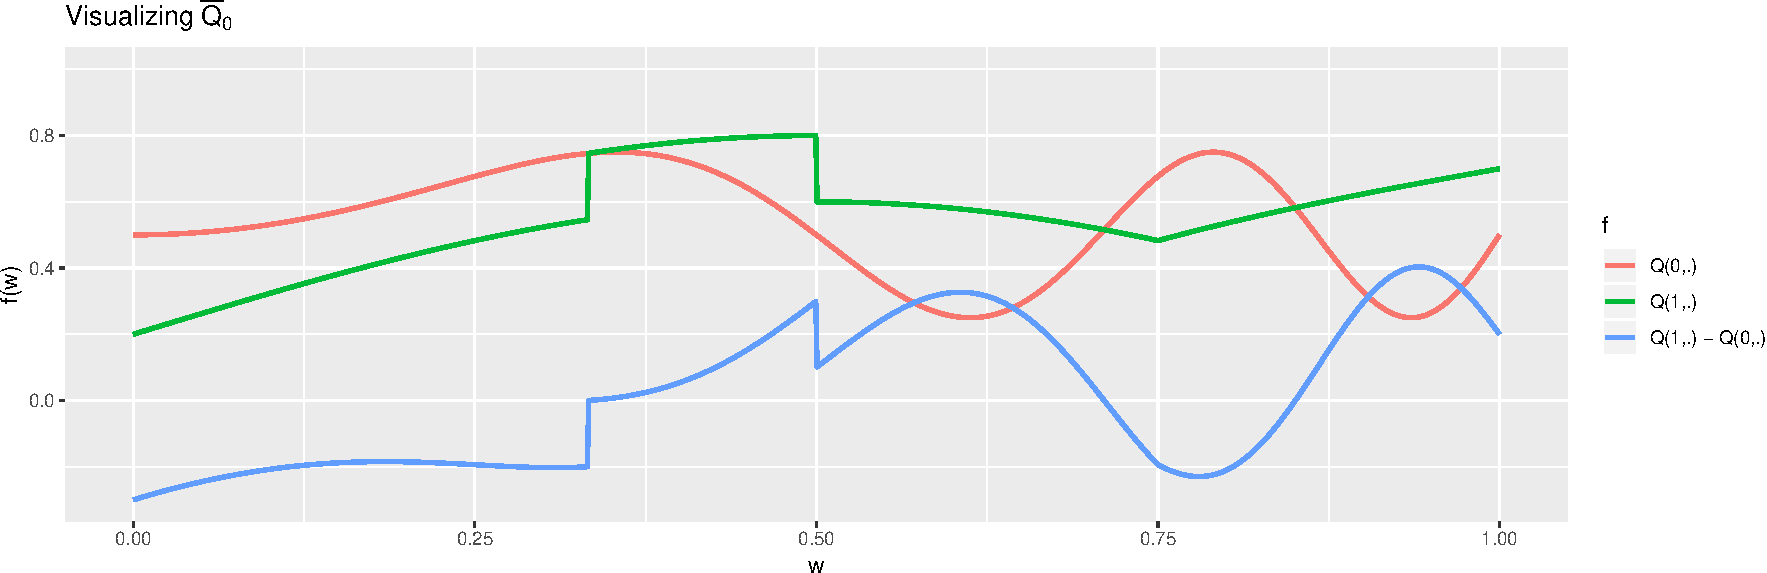
\includegraphics{img/exercise:visualize-1.pdf}

\begin{enumerate}
\def\labelenumi{\arabic{enumi}.}
\setcounter{enumi}{1}
\tightlist
\item
  Adapt the above chunk of code to visualize the marginal density
  \(Q_{0,W}\) and conditional probability \(\Gbar_{0}\).
\end{enumerate}

\subsection{The parameter of interest, first pass.}
\label{subsec:parameter:first}

It happens that we especially care for a finite-dimensional feature of
\(P_{0}\) that we denote by \(\psi_{0}\). Its definition involves two of
the aforementioned infinite-dimensional features:
\begin{align}  \label{eq:psi0}
\psi_{0}  &\equiv   \int  \left(\Qbar_{0}(1,   w)  -   \Qbar_{0}(0,  w)\right)
dQ_{0,W}(w)\\  \notag  &=  \Exp_{P_{0}}   \left(\Exp_{P_0}(Y \mid A = 1,  W)  -  \Exp_{P_0}(Y \mid A = 0,  W) \right).   \end{align}
Acting as oracles, we can compute explicitly the numerical value of
\(\psi_{0}\).

\begin{Shaded}
\begin{Highlighting}[]
\NormalTok{integrand <-}\StringTok{ }\ControlFlowTok{function}\NormalTok{(w) \{}
\NormalTok{  Qbar <-}\StringTok{ }\KeywordTok{attr}\NormalTok{(five_obs, }\StringTok{"Qbar"}\NormalTok{)}
\NormalTok{  QW <-}\StringTok{ }\KeywordTok{attr}\NormalTok{(five_obs, }\StringTok{"QW"}\NormalTok{)}
\NormalTok{  ( }\KeywordTok{Qbar}\NormalTok{(}\KeywordTok{cbind}\NormalTok{(}\DecValTok{1}\NormalTok{, w)) }\OperatorTok{-}\StringTok{ }\KeywordTok{Qbar}\NormalTok{(}\KeywordTok{cbind}\NormalTok{(}\DecValTok{0}\NormalTok{, w)) ) }\OperatorTok{*}\StringTok{ }\KeywordTok{QW}\NormalTok{(w)}
\NormalTok{\}}
\NormalTok{(psi_zero <-}\StringTok{ }\KeywordTok{integrate}\NormalTok{(integrand, }\DataTypeTok{lower =} \DecValTok{0}\NormalTok{, }\DataTypeTok{upper =} \DecValTok{1}\NormalTok{)}\OperatorTok{$}\NormalTok{val)}
\end{Highlighting}
\end{Shaded}

\begin{verbatim}
## [1] 0.08317711
\end{verbatim}

Our interest in \(\psi_{0}\) is of causal nature. Taking a closer look
at \texttt{drawFromExperiment} reveals indeed that the random making of
an observation \(O\) drawn from \(P_{0}\) can be summarized by the
following causal graph and nonparametric system of structural equations:

\begin{Shaded}
\begin{Highlighting}[]
\NormalTok{## plot the causal diagram}
\end{Highlighting}
\end{Shaded}

and, for some deterministic functions \(f_w\), \(f_a\), \(f_y\) and
independent sources of randomness \(U_w\), \(U_a\), \(U_y\),

\begin{enumerate}
\item sample  the context where the  rest of the experiment
  will take place \tcg{Not sure I understand this sentence}, $W = f_{w}(U_w)$;
\item  sample the  two counterfactual  rewards of  the two
  actions  that   can  be   undertaken,  $Y_{0}  =   f_{y}(0,  W,   U_y)$  and
  $Y_{1} = f_{y}(1, W, U_y)$;
\item\label{item:A:equals} sample   which  action is carried
  out in the given context, $A = f_{a} (W, U_a)$;
\item    define        the    corresponding    reward,
  $Y = A Y_{1} + (1-A) Y_{0}$;
\item summarize the course of the experiment  with the observation $O = (W, A,
  Y)$, thus concealing $Y_{0}$ and $Y_{1}$. 
\end{enumerate}

The above description of the experiment \texttt{draw\_from\_experiment}
is useful to reinforce what it means to run the ``ideal'' experiment by
setting argument \texttt{ideal} to \texttt{TRUE} in a call to
\texttt{draw\_from\_experiment}. Doing so triggers a modification of the
nature of the experiment, enforcing that the counterfactual rewards
\(Y_{0}\) and \(Y_{1}\) be part of the summary of the experiment
eventually. In light of the above enumeration,
\(\bbO \equiv (W, Y_{0}, Y_{1}, A, Y)\) is output, as opposed to its
summary measure \(O\). This defines another experiment and its law, that
we denote \(\bbP_{0}\).

It is straightforward to show\footnote{For $a = 0,1$, $$
E(Y_a) = \int \Exp_{\bbP_0}(Y_a \mid W = w) dQ_{0,W}(w) = \int \Exp_{\bbP_0}(Y_a \mid A = a, W = w) dQ_{0,W}(w) = \int \Exp_{P_0}(Y \mid A = a, W = w) dQ_{0,W}(w) = \int \Qbar_0(a,W) dQ_{0,W}(w). 
$$} that under assumptions\footnote{Something}
\begin{equation} \label{eq:psi:zero}    
\psi_{0} = \Exp_{\bbP_{0}} \left(Y_{1} - Y_{0}\right) = \Exp_{\bbP_{0}}(Y_1) -
\Exp_{\bbP_{0}}(Y_0).  \end{equation} Thus, \(\psi_{0}\) describes the
average difference in of the two counterfactual rewards. In other words,
\(\psi_{0}\) quantifies the difference in average of the reward one
would get in a world where one would always enforce action \(a=1\) with
the reward one would get in a world where one would always enforce
action \(a=0\). This said, it is worth emphasizing that \(\psi_{0}\) is
a well defined parameter beyond its causal interpretation.

To conclude this subsection, we take advantage of our position as
oracles to sample observations from the ideal experiment. We call
\texttt{draw\_from\_experiment} with its argument \texttt{ideal} set to
\texttt{TRUE} in order to numerically approximate \(\psi_{0}\). By the
law of large numbers, the following chunk of code approximates
\(\psi_{0}\) and shows it approximate value:

\begin{Shaded}
\begin{Highlighting}[]
\NormalTok{B <-}\StringTok{ }\FloatTok{1e6}\NormalTok{ ## Antoine: 1e6 eventually}
\NormalTok{ideal_obs <-}\StringTok{ }\KeywordTok{draw_from_experiment}\NormalTok{(B, }\DataTypeTok{ideal =} \OtherTok{TRUE}\NormalTok{)}
\NormalTok{(psi_approx <-}\StringTok{ }\KeywordTok{mean}\NormalTok{(ideal_obs[, }\StringTok{"Yone"}\NormalTok{] }\OperatorTok{-}\StringTok{ }\NormalTok{ideal_obs[, }\StringTok{"Yzero"}\NormalTok{]))}
\end{Highlighting}
\end{Shaded}

\begin{verbatim}
## [1] 0.08293116
\end{verbatim}

In fact, the central limit theorem and Slutsky's lemma allow us to build
a confidence interval with asymptotic level 95\% for \(\psi_{0}\):

\begin{Shaded}
\begin{Highlighting}[]
\NormalTok{sd_approx <-}\StringTok{ }\KeywordTok{sd}\NormalTok{(ideal_obs[, }\StringTok{"Yone"}\NormalTok{] }\OperatorTok{-}\StringTok{ }\NormalTok{ideal_obs[, }\StringTok{"Yzero"}\NormalTok{])}
\NormalTok{alpha <-}\StringTok{ }\FloatTok{0.05}
\NormalTok{(psi_approx_CI <-}\StringTok{ }\NormalTok{psi_approx }\OperatorTok{+}\StringTok{ }\KeywordTok{c}\NormalTok{(}\OperatorTok{-}\DecValTok{1}\NormalTok{, }\DecValTok{1}\NormalTok{) }\OperatorTok{*}\StringTok{ }\KeywordTok{qnorm}\NormalTok{(}\DecValTok{1} \OperatorTok{-}\StringTok{ }\NormalTok{alpha }\OperatorTok{/}\StringTok{ }\DecValTok{2}\NormalTok{) }\OperatorTok{*}\StringTok{ }\NormalTok{sd_approx }\OperatorTok{/}\StringTok{ }\KeywordTok{sqrt}\NormalTok{(B))}
\end{Highlighting}
\end{Shaded}

\begin{verbatim}
## [1] 0.08232477 0.08353754
\end{verbatim}

\subsection{\gear Difference in covariate-adjusted quantile rewards, first
pass.}  
\label{subsec:exo:dave:one}

The problems come within the scope of Sections
\ref{subsec:parameter:first}.

As discussed above, parameter \(\psi_0\) \eqref{eq:psi:zero} is the
difference in average rewards if we enforce action \(a = 1\) rather than
\(a = 0\). An alternative way to describe the rewards under different
actions involves quantiles as opposed to averages.

Let \(Q_{0,Y}(y, a, w) = \int_{0}^y q_{0,Y}(u, a, w) du\) be the
conditional cumulative distribution of reward \(Y\) given \(A=a\) and
\(W=w\), evaluated at \(y \in \interval[open]{0}{1}\), that is implied
by \(P_0\). For each action \(a \in \{0,1\}\) and
\(c \in \interval[open]{0}{1}\), introduce \begin{equation}
\label{def_quantile}     \gamma_{0,a,c}    \equiv     \inf    \left\{y     \in
\interval[open]{0}{1}  : \int  Q_{0,Y}(y, a,  w) dQ_{0,W}(w)  \ge c  \right\}.
\end{equation}

It is not difficult to check that
\tcg{do  we give the proof or refer to other
articles?}
\begin{equation*}\gamma_{0,a,c}     =     \inf\left\{y     \in
\interval[open]{0}{1}      :      \Pr_{\bbP_{0}}(Y_a     \leq      y)      \geq
c\right\}.\end{equation*} Thus, \(\gamma_{0,a,c}\) can be interpreted as
a covariate-adjusted \(c\)-th quantile reward when action \(a\) is
enforced. The difference
\begin{equation*}\delta_{0,c}    \equiv     \gamma_{0,1,c}    -
\gamma_{0,0,c}\end{equation*} is the \(c\)-th quantile counterpart to
parameter \(\psi_{0}\) \eqref{eq:psi:zero}.

\begin{enumerate}
\def\labelenumi{\arabic{enumi}.}
\item
  \textdbend Compute the numerical value of \(\gamma_{0,a,c}\) for each
  \((a,c) \in \{0,1\} \times \{1/4, 1/2, 3/4\}\) using the appropriate
  attributes of \texttt{five\_obs}. Based on these results, report the
  numerical value of \(\delta_{0,c}\) for each
  \(c \in \{1/4, 1/2, 3/4\}\).
\item
  Approximate the numerical values of \(\gamma_{0,a,c}\) for each
  \((a,c) \in \{0,1\} \times \{1/4, 1/2, 3/4\}\) by drawing a large
  sample from the ``ideal'' data experiment and using empirical quantile
  estimates. Deduce from these results a numerical approximation to
  \(\delta_{0,c}\) for \(c \in \{1/4, 1/2, 3/4\}\). Confirm that your
  results closely match those obtained in the previous problem.
\end{enumerate}

\subsection{The parameter of interest, second pass.}
\label{subsec:parameter:second}

Suppose we know beforehand that \(O\) drawn from \(P_{0}\) takes its
values in \(\calO \equiv [0,1] \times \{0,1\} \times \interval{0}{1}\)
and that \(\Gbar(W) = P_{0}(A=1|W)\) is bounded away from zero and one
\(Q_{0,W}\)-almost surely (this is the case indeed). Then we can define
model \(\calM\) as the set of all laws \(P\) on \(\calO\) such that
\(\Gbar(W) \equiv P(A=1|W)\) is bounded away from zero and one
\(Q_{W}\)-almost surely, where \(Q_{W}\) is the marginal law of \(W\)
under \(P\).

Let us also define generically \(\Qbar\) as
\begin{equation*} \Qbar (A,W) \equiv
\Exp_{P}  (Y|A,  W).   \end{equation*} Central to our approach is
viewing \(\psi_{0}\) as the value at \(P_{0}\) of the statistical
mapping \(\Psi\) from \(\calM\) to \([0,1]\) characterized by
\begin{align*}  \Psi(P)  &\equiv  \int
\left(\Qbar(1, w) - \Qbar(0, w)\right) dQ_{W}(w) \\ &= \Exp_{P} \left(\Qbar(1,
W) -  \Qbar(0, W)\right), \end{align*} a clear extension of
\eqref{eq:psi0}. For instance, although the law \(\Pi_{0} \in \calM\)
encoded by default (\textit{i.e.}, with \texttt{h=0}) in
\texttt{drawFromAnotherExperiment} defined below differs starkly from
\(P_{0}\),

\begin{Shaded}
\begin{Highlighting}[]
\NormalTok{draw_from_another_experiment <-}\StringTok{ }\ControlFlowTok{function}\NormalTok{(n, }\DataTypeTok{h =} \DecValTok{0}\NormalTok{) \{}
\NormalTok{  ## preliminary}
\NormalTok{  n <-}\StringTok{ }\NormalTok{Arguments}\OperatorTok{$}\KeywordTok{getInteger}\NormalTok{(n, }\KeywordTok{c}\NormalTok{(}\DecValTok{1}\NormalTok{, }\OtherTok{Inf}\NormalTok{))}
\NormalTok{  h <-}\StringTok{ }\NormalTok{Arguments}\OperatorTok{$}\KeywordTok{getNumeric}\NormalTok{(h)}
\NormalTok{  ## ## 'Gbar' and 'Qbar' factors}
\NormalTok{  Gbar <-}\StringTok{ }\ControlFlowTok{function}\NormalTok{(W) \{}
    \KeywordTok{sin}\NormalTok{((}\DecValTok{1} \OperatorTok{+}\StringTok{ }\NormalTok{W) }\OperatorTok{*}\StringTok{ }\NormalTok{pi }\OperatorTok{/}\StringTok{ }\DecValTok{6}\NormalTok{)}
\NormalTok{  \}}
\NormalTok{  Qbar <-}\StringTok{ }\ControlFlowTok{function}\NormalTok{(AW, }\DataTypeTok{hh =}\NormalTok{ h) \{}
\NormalTok{    A <-}\StringTok{ }\NormalTok{AW[, }\DecValTok{1}\NormalTok{]}
\NormalTok{    W <-}\StringTok{ }\NormalTok{AW[, }\DecValTok{2}\NormalTok{]}
    \KeywordTok{expit}\NormalTok{( }\KeywordTok{logit}\NormalTok{( A }\OperatorTok{*}\StringTok{  }\NormalTok{W }\OperatorTok{+}\StringTok{ }\NormalTok{(}\DecValTok{1} \OperatorTok{-}\StringTok{ }\NormalTok{A) }\OperatorTok{*}\StringTok{ }\NormalTok{W}\OperatorTok{^}\DecValTok{2}\NormalTok{ ) }\OperatorTok{+}
\StringTok{           }\NormalTok{hh }\OperatorTok{*}\StringTok{ }\DecValTok{10} \OperatorTok{*}\StringTok{ }\KeywordTok{sqrt}\NormalTok{(W) }\OperatorTok{*}\StringTok{ }\NormalTok{A )}
\NormalTok{  \}}
\NormalTok{  ## sampling}
\NormalTok{  ## ## context}
\NormalTok{  W <-}\StringTok{ }\KeywordTok{runif}\NormalTok{(n, }\DataTypeTok{min =} \DecValTok{1}\OperatorTok{/}\DecValTok{10}\NormalTok{, }\DataTypeTok{max =} \DecValTok{9}\OperatorTok{/}\DecValTok{10}\NormalTok{)}
\NormalTok{  ## ## action undertaken}
\NormalTok{  A <-}\StringTok{ }\KeywordTok{rbinom}\NormalTok{(n, }\DataTypeTok{size =} \DecValTok{1}\NormalTok{, }\DataTypeTok{prob =} \KeywordTok{Gbar}\NormalTok{(W))}
\NormalTok{  ## ## reward}
\NormalTok{  shape1 <-}\StringTok{ }\DecValTok{4}
\NormalTok{  QAW <-}\StringTok{ }\KeywordTok{Qbar}\NormalTok{(}\KeywordTok{cbind}\NormalTok{(A, W))}
\NormalTok{  Y <-}\StringTok{ }\KeywordTok{rbeta}\NormalTok{(n, }\DataTypeTok{shape1 =}\NormalTok{ shape1, }\DataTypeTok{shape2 =}\NormalTok{ shape1 }\OperatorTok{*}\StringTok{ }\NormalTok{(}\DecValTok{1} \OperatorTok{-}\StringTok{ }\NormalTok{QAW) }\OperatorTok{/}\StringTok{ }\NormalTok{QAW)}
\NormalTok{  ## ## observation}
\NormalTok{  obs <-}\StringTok{ }\KeywordTok{cbind}\NormalTok{(}\DataTypeTok{W =}\NormalTok{ W, }\DataTypeTok{A =}\NormalTok{ A, }\DataTypeTok{Y =}\NormalTok{ Y)}
  \KeywordTok{attr}\NormalTok{(obs, }\StringTok{"Gbar"}\NormalTok{) <-}\StringTok{ }\NormalTok{Gbar}
  \KeywordTok{attr}\NormalTok{(obs, }\StringTok{"Qbar"}\NormalTok{) <-}\StringTok{ }\NormalTok{Qbar}
  \KeywordTok{attr}\NormalTok{(obs, }\StringTok{"QW"}\NormalTok{) <-}\StringTok{ }\ControlFlowTok{function}\NormalTok{(x)\{}\KeywordTok{dunif}\NormalTok{(x, }\DataTypeTok{min =} \DecValTok{1}\OperatorTok{/}\DecValTok{10}\NormalTok{, }\DataTypeTok{max =} \DecValTok{9}\OperatorTok{/}\DecValTok{10}\NormalTok{)\}}
  \KeywordTok{attr}\NormalTok{(obs, }\StringTok{"shape1"}\NormalTok{) <-}\StringTok{ }\NormalTok{shape1}
  \KeywordTok{attr}\NormalTok{(obs, }\StringTok{"qY"}\NormalTok{) <-}\StringTok{ }\ControlFlowTok{function}\NormalTok{(AW, Y, Qbar, shape1)\{}
\NormalTok{    A <-}\StringTok{ }\NormalTok{AW[,}\DecValTok{1}\NormalTok{]; W <-}\StringTok{ }\NormalTok{AW[,}\DecValTok{2}\NormalTok{]}
\NormalTok{    Qbar.AW <-}\StringTok{ }\KeywordTok{do.call}\NormalTok{(Qbar, }\KeywordTok{list}\NormalTok{(AW))}
    \KeywordTok{dbeta}\NormalTok{(Y, }\DataTypeTok{shape1 =}\NormalTok{ shape1, }\DataTypeTok{shape2 =}\NormalTok{ shape1 }\OperatorTok{*}\StringTok{ }\NormalTok{(}\DecValTok{1} \OperatorTok{-}\StringTok{ }\NormalTok{Qbar.AW) }\OperatorTok{/}\StringTok{ }\NormalTok{Qbar.AW)}
\NormalTok{  \}}
\NormalTok{  ##}
  \KeywordTok{return}\NormalTok{(obs)}
\NormalTok{\}}
\end{Highlighting}
\end{Shaded}

the parameter \(\Psi(\Pi_{0})\) is well defined, and numerically
approximated by \texttt{psi\_Pi\_zero} as follows.

\begin{Shaded}
\begin{Highlighting}[]
\NormalTok{five_obs_from_another_experiment <-}\StringTok{ }\KeywordTok{draw_from_another_experiment}\NormalTok{(}\DecValTok{5}\NormalTok{)}
\NormalTok{another_integrand <-}\StringTok{ }\ControlFlowTok{function}\NormalTok{(w) \{}
\NormalTok{  Qbar <-}\StringTok{ }\KeywordTok{attr}\NormalTok{(five_obs_from_another_experiment, }\StringTok{"Qbar"}\NormalTok{)}
\NormalTok{  QW <-}\StringTok{ }\KeywordTok{attr}\NormalTok{(five_obs_from_another_experiment, }\StringTok{"QW"}\NormalTok{)}
\NormalTok{  ( }\KeywordTok{Qbar}\NormalTok{(}\KeywordTok{cbind}\NormalTok{(}\DecValTok{1}\NormalTok{, w)) }\OperatorTok{-}\StringTok{ }\KeywordTok{Qbar}\NormalTok{(}\KeywordTok{cbind}\NormalTok{(}\DecValTok{0}\NormalTok{, w)) ) }\OperatorTok{*}\StringTok{ }\KeywordTok{QW}\NormalTok{(w)}
\NormalTok{\}}
\NormalTok{(psi_Pi_zero <-}\StringTok{ }\KeywordTok{integrate}\NormalTok{(another_integrand, }\DataTypeTok{lower =} \DecValTok{0}\NormalTok{, }\DataTypeTok{upper =} \DecValTok{1}\NormalTok{)}\OperatorTok{$}\NormalTok{val)}
\end{Highlighting}
\end{Shaded}

\begin{verbatim}
## [1] 0.1966687
\end{verbatim}

Straightforward algebra confirms that indeed \(\Psi(\Pi_{0}) = 59/300\).

\subsection{\gear  Difference in  covariate-adjusted quantile  rewards, second
pass.}  
\label{subsec:exo:dave:two}

We continue with the exercise from Section \ref{subsec:exo:dave:one}.
The problems come within the scope of Section
\ref{subsec:parameter:first}.

As above, we define \(q_{Y}(y,a,w)\) to be the \((A,W)\)-conditional
density of \(Y\) given \(A=a\) and \(W=w\), evaluated at \(y\), that is
implied by a generic \(P \in \calM\). Similarly, we use \(Q_{Y}\) to
denote the corresponding cumulative distribution function. The
covariate-adjusted \(c\)-th quantile reward for action \(a \in \{0,1\}\)
may be viewed as a mapping \(\Gamma_{a,c}\) from \(\calM\) to \([0,1]\)
characterized by \begin{equation*} \Gamma_{a,c}(P)  = \inf\left\{y
\in  \interval[open]{0}{1}  :  \int   Q_{Y}(y,a,w)  dQ_W(w)  \ge  c  \right\}.
\end{equation*} The difference in \(c\)-th quantile rewards may
similarly be viewed as a mapping \(\Delta_c\) from \(\calM\) to
\([0,1]\), characterized by
\(\Delta_c(P) \equiv \Gamma_{1,c}(P) - \Gamma_{0,c}(P)\).

\begin{enumerate}
\def\labelenumi{\arabic{enumi}.}
\item
  Compute the numerical value of \(\Gamma_{a,c}(\Pi_0)\) for
  \((a,c) \in \{0,1\} \times \{1/4, 1/2, 3/4\}\) using the appropriate
  attributes of \texttt{five\_obs\_from\_another\_experiment}. Based on
  these results, report the numerical value of \(\Delta_c(\Pi_0)\) for
  each \(c \in \{1/4, 1/2, 3/4\}\).
\item
  Approximate the value of \(\Gamma_{0,a,c}(\Pi_{0})\) for
  \((a,c) \in \{0,1\} \times \{1/4, 1/2, 3/4\}\) by drawing a large
  sample from the ``ideal'' data experiment and using empirical quantile
  estimates. Deduce from these results a numerical approximation to
  \(\Delta_{0,c} (\Pi_{0})\) for each \(c \in \{1/4, 1/2, 3/4\}\).
  Confirm that your results closely match those obtained in the previous
  problem.
\item
  Building upon the code you wrote to solve the previous problem,
  construct a confidence interval with asymptotic level \(95\%\) for
  \(\Delta_{0,c} (\Pi_{0})\), with
  \(c \in \{1/4, 1/2, 3/4\}\).\footnote{Let  $X_{1}, \ldots,
  X_{n}$  be  independently drawn  from  a  continuous distribution  function
  $F$. Set  $p \in  \interval[open]{0}{1}$ and, assuming  that $n$  is large,
  find   $k\geq  1$   and  $l   \geq   1$  such   that  $k/n   \approx  p   -
  \Phi^{-1}(1-\alpha)    \sqrt{p(1-p)/n}$    and    $l/n    \approx    p    +
  \Phi^{-1}(1-\alpha) \sqrt{p(1-p)/n}$,  where $\Phi$ is the  standard normal
  distribution function.  Then  $\interval{X_{(k)}}{X_{(l)}}$ is a confidence
  interval for $F^{-1}(p)$ with asymptotic level $1 - 2\alpha$.}
\end{enumerate}

\subsection{The parameter of interest, third pass.}
\label{subsec:parameter:third}

In the previous subsection, we reoriented our view of the target
parameter to be a statistical functional of the distribution of the
observed data. Specifically, we viewed the parameter as a function of
specific features of the observed data distribution, namely \(Q_{W}\)
and \(\Qbar\). It is straightforward\footnote{
  For $a = 0,1$, \begin{align*}
    \Exp_{P_0}\left(\frac{I(A = a)Y}{\ell\Gbar{a,W}}\right) &= \Exp_{P_0}\left\{\Exp_{P_0}\left(\frac{I(A = a)Y}{\ell\Gbar{a,W}} \mid A, W\right) \right\} = \Exp_{P_0}\left\{\frac{I(A = a)}{\ell\Gbar{a,W}} \Exp_{P_0}(Y \mid A, W) \right\} \\
    &= \Exp_{P_0}\left\{\frac{I(A = a)}{\ell\Gbar{a,W}} \Exp_{P_0}(Y \mid A = 1, W) \right\} 
    = \Exp_{P_0}\left\{\Exp_{P_0}\left(\frac{I(A = a)}{\ell\Gbar{a,W}} \Exp_{P_0}(Y \mid A = 1, W) \mid W \right) \right\} \\
    &=  \Exp_{P_0}\left(\ell\Gbar{a,W}}{\ell\Gbar{a,W}} \Exp_{P_0}(Y \mid A = 1, W) \mid W \right) = \Exp_{P_0} \left( \Exp_{P_0}(Y \mid A = 1, W) \right) \ . 
    \end{align*}
} to show an equivalent representation of the parameter as
\begin{equation}\label{eq:psi0:b} 
\psi_{0} = \Exp_{P_{0}}    \left\{\frac{I(A = 1)}{\ell\Gbar_{0}(1,W)} - \frac{I(A = 0)}{\ell\Gbar_{0}(0,W)} \right) Y \right\}   \ , 
\end{equation} or, viewing the parameter as a statistical functional,
for a given \(P\) in the model \begin{equation} \label{eq:psi0:c}
\Psi(P) = \Exp_{P}\left\{\frac{I(A = 1)}{\mbox{Pr}_P(A = 1 \mid W)} - \frac{I(A = 0)}{\mbox{Pr}_P(A = 1 \mid W)} \right) Y \right\} \ . 
\end{equation}

\subsection{Being smooth, first pass.}
\label{subsec:being:smooth:one}

Luckily, the statistical mapping \(\Psi\) is well behaved, or smooth.
Here, this colloquial expression refers to the fact that, for each
\(P \in \calM\), if \(P_{h} \to_{h} P\) in \(\calM\) from a direction
\(s\) when the real parameter \(h \to 0\), then not only
\(\Psi(P_{h}) \to_{h} \Psi(P)\) (continuity), but also
\(h^{-1} [\Psi(P_{h}) - \Psi(P)] \to_{h} c\), where the real number
\(c\) depends on \(P\) and \(s\) (differentiability).

For instance, let \(\Pi_{h} \in \calM\) be the law encoded in
\texttt{draw\_from\_another\_experiment} with \texttt{h} ranging over
\(\interval{-1}{1}\). We will argue shortly that
\(\Pi_{h} \to_{h} \Pi_{0}\) in \(\calM\) from a direction \(s\) when
\(h \to 0\). The following chunk of code evaluates and represents
\(\Psi(\Pi_{h})\) for \(h\) ranging in a discrete approximation of
\(\interval{-1}{1}\):

\begin{Shaded}
\begin{Highlighting}[]
\NormalTok{approx <-}\StringTok{ }\KeywordTok{seq}\NormalTok{(}\OperatorTok{-}\DecValTok{1}\NormalTok{, }\DecValTok{1}\NormalTok{, }\DataTypeTok{length.out =} \FloatTok{1e2}\NormalTok{)}
\NormalTok{psi_Pi_h <-}\StringTok{ }\KeywordTok{sapply}\NormalTok{(approx, }\ControlFlowTok{function}\NormalTok{(t) \{}
\NormalTok{  obs_from_another_experiment <-}\StringTok{ }\KeywordTok{draw_from_another_experiment}\NormalTok{(}\DecValTok{1}\NormalTok{, }\DataTypeTok{h =}\NormalTok{ t)}
\NormalTok{  integrand <-}\StringTok{ }\ControlFlowTok{function}\NormalTok{(w) \{}
\NormalTok{    Qbar <-}\StringTok{ }\KeywordTok{attr}\NormalTok{(obs_from_another_experiment, }\StringTok{"Qbar"}\NormalTok{)}
\NormalTok{    QW <-}\StringTok{ }\KeywordTok{attr}\NormalTok{(obs_from_another_experiment, }\StringTok{"QW"}\NormalTok{)}
\NormalTok{    ( }\KeywordTok{Qbar}\NormalTok{(}\KeywordTok{cbind}\NormalTok{(}\DecValTok{1}\NormalTok{, w)) }\OperatorTok{-}\StringTok{ }\KeywordTok{Qbar}\NormalTok{(}\KeywordTok{cbind}\NormalTok{(}\DecValTok{0}\NormalTok{, w)) ) }\OperatorTok{*}\StringTok{ }\KeywordTok{QW}\NormalTok{(w)}
\NormalTok{  \}}
  \KeywordTok{integrate}\NormalTok{(integrand, }\DataTypeTok{lower =} \DecValTok{0}\NormalTok{, }\DataTypeTok{upper =} \DecValTok{1}\NormalTok{)}\OperatorTok{$}\NormalTok{val  }
\NormalTok{\})}
\NormalTok{slope_approx <-}\StringTok{ }\NormalTok{(psi_Pi_h }\OperatorTok{-}\StringTok{ }\NormalTok{psi_Pi_zero) }\OperatorTok{/}\StringTok{ }\NormalTok{approx}
\NormalTok{slope_approx <-}\StringTok{ }\NormalTok{slope_approx[}\KeywordTok{min}\NormalTok{(}\KeywordTok{which}\NormalTok{(approx }\OperatorTok{>}\StringTok{ }\DecValTok{0}\NormalTok{))]}
\KeywordTok{ggplot}\NormalTok{() }\OperatorTok{+}
\StringTok{  }\KeywordTok{geom_point}\NormalTok{(}\DataTypeTok{data =} \KeywordTok{data.frame}\NormalTok{(}\DataTypeTok{x =}\NormalTok{ approx, }\DataTypeTok{y =}\NormalTok{ psi_Pi_h), }\KeywordTok{aes}\NormalTok{(x, y),}
             \DataTypeTok{color =} \StringTok{"#CC6666"}\NormalTok{) }\OperatorTok{+}
\StringTok{  }\KeywordTok{geom_segment}\NormalTok{(}\KeywordTok{aes}\NormalTok{(}\DataTypeTok{x =} \DecValTok{-1}\NormalTok{, }\DataTypeTok{y =}\NormalTok{ psi_Pi_zero }\OperatorTok{-}\StringTok{ }\NormalTok{slope_approx,}
                   \DataTypeTok{xend =} \DecValTok{1}\NormalTok{, }\DataTypeTok{yend =}\NormalTok{ psi_Pi_zero }\OperatorTok{+}\StringTok{ }\NormalTok{slope_approx),}
               \DataTypeTok{arrow =} \KeywordTok{arrow}\NormalTok{(}\DataTypeTok{length =} \KeywordTok{unit}\NormalTok{(}\FloatTok{0.03}\NormalTok{, }\StringTok{"npc"}\NormalTok{)),}
               \DataTypeTok{color =} \StringTok{"#9999CC"}\NormalTok{) }\OperatorTok{+}
\StringTok{  }\KeywordTok{geom_vline}\NormalTok{(}\DataTypeTok{xintercept =} \DecValTok{0}\NormalTok{, }\DataTypeTok{color =} \StringTok{"#66CC99"}\NormalTok{) }\OperatorTok{+}
\StringTok{  }\KeywordTok{geom_hline}\NormalTok{(}\DataTypeTok{yintercept =}\NormalTok{ psi_Pi_zero, }\DataTypeTok{color =} \StringTok{"#66CC99"}\NormalTok{) }\OperatorTok{+}
\StringTok{  }\KeywordTok{labs}\NormalTok{(}\DataTypeTok{x =} \StringTok{"h"}\NormalTok{, }\DataTypeTok{y =} \KeywordTok{expression}\NormalTok{(}\KeywordTok{Psi}\NormalTok{(Pi[h]))) }
\end{Highlighting}
\end{Shaded}

\begin{figure}
\centering
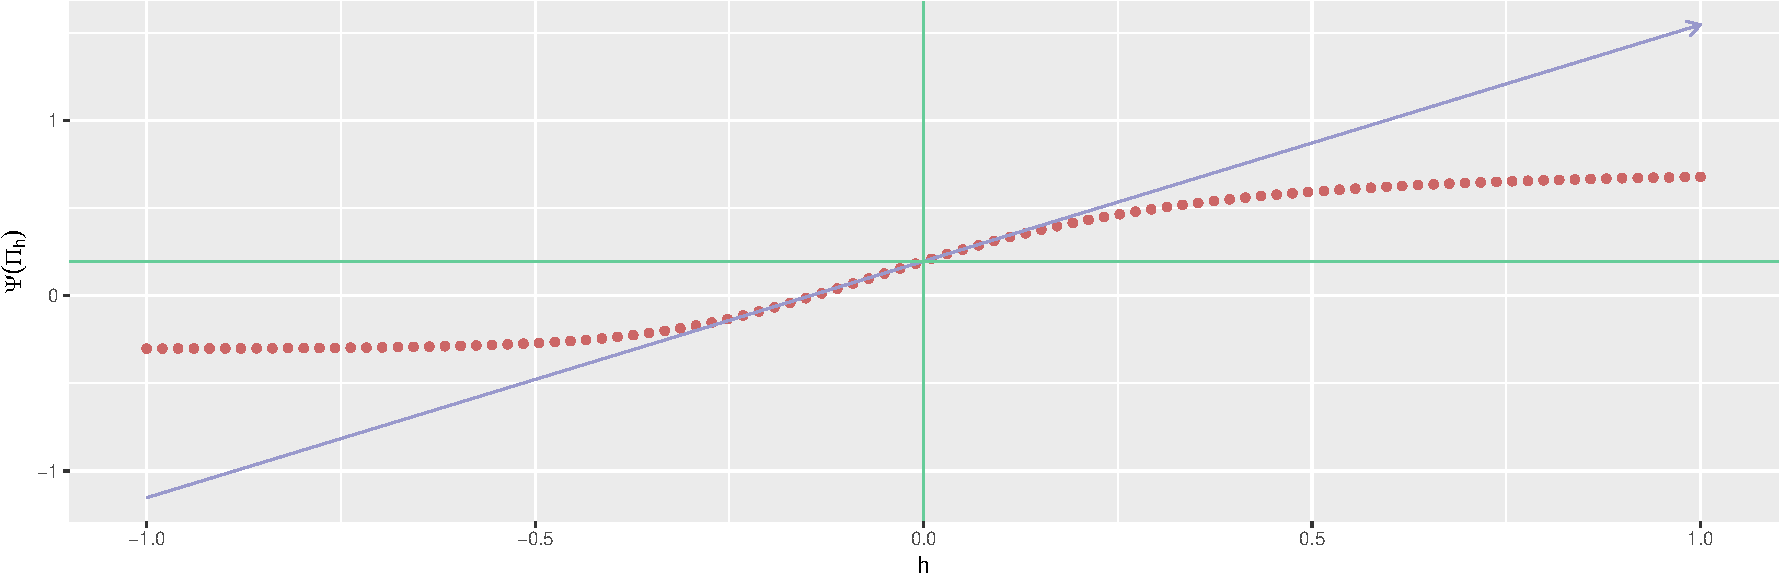
\includegraphics{img/psi-approx-psi-one-1.pdf}
\caption{\label{fig:psi-approx-psi-one}Evolution of statistical parameter
\(\Psi\) along fluctuation \(\{\Pi_{h} : h \in H\}\).}
\end{figure}

The dotted curve represents the function \(h \mapsto \Psi(\Pi_{h})\).
The blue line represents the tangent to the previous curve at \(h=0\),
which is indeed differentiable around \(h=0\). It is derived by simple
geometric arguments. In the next subsection, we formalize what it means
to be smooth for the statistical mapping \(\Psi\). Once the presentation
is complete, we will be able to derive a closed-form expression for the
slope of the blue curve from the chunk of code where
\texttt{draw\_from\_another\_experiment} is defined.

\subsection{\textdbend Being smooth, second pass.}
\label{subsec:being:smooth:two}

Let us now describe what it means for statistical mapping \(\Psi\) to be
smooth at every \(P \in \calM\). The description necessitates the
introduction of fluctuations.

For every direction\footnote{A direction is a measurable function.}
\(s : \calO \to \bbR\) such that
\(s \neq 0\)\footnote{That is, $s(O)$ is  not equal to zero
$P$-almost surely.}, \(\Exp_{P} (s(O)) = 0\) and \(s\) bounded by, say,
\(M\), for every \(h \in H \equiv \interval[open]{-M^{-1}}{M^{-1}}\), we
can define a law \(P_{h} \in \calM\) by setting
\(P_{h} \ll P\)\footnote{That  is, $P_{h}$  is
dominated  by $P$:  if an  event $A$  satisfies $P(A)  = 0$,  then necessarily
$P_{h} (A) = 0$ too.} and

\begin{equation}\label{eq:fluct}\frac{dP_{h}}{dP}(O)    \equiv     1    +    h
s(O),\end{equation}

that is, \(P_{h}\) has density \((1 + h s)\) with respect to (w.r.t.)
\(P\). We call \(\{P_{h} : h \in H\}\) a fluctuation of \(P\) in
direction \(s\) because

\begin{equation}\label{eq:score}(i)  \;  P_{h}|_{h=0}  =   P,  \quad  (ii)  \;
\left.\frac{d}{dh}       \log        \frac{dP_{h}}{dP}(O)\right|_{h=0}       =
s(O).\end{equation}

The fluctuation is a one-dimensional parametric submodel of \(\calM\).

Statistical mapping \(\Psi\) is smooth at every \(P \in \calM\) because,
for each \(P \in \calM\), there exists a so called efficient influence
curve\footnote{It
is  a   measurable  function.} \(D^{*}(P) : \calO \to \bbR\) such that
\(\Exp_{P}(D^{*}(P)(O)) = 0\) and, for any direction \(s\) as above, if
\(\{P_{h} : h \in H\}\) is defined as in \eqref{eq:fluct}, then the
real-valued mapping \(h \mapsto \Psi(P_{h})\) is differentiable at
\(h=0\), with a derivative equal to

\begin{equation}\label{eq:derivative}\Exp_{P}                \left(D^{*}(P)(O)
s(O)\right).\end{equation}

Interestingly, if a fluctuation \(\{P_{h} : h \in H\}\) satisfies
\eqref{eq:score} for a direction \(s\) such that \(s\neq 0\),
\(\Exp_{P}(s(O)) = 0\) and \(\Var_{P} (s(O)) < \infty\), then
\(h \mapsto \Psi(P_{h})\) is still differentiable at \(h=0\) with a
derivative equal to \eqref{eq:derivative} (beyond fluctuations of the
form \eqref{eq:fluct}).

The influence curves \(D^{*}(P)\) convey valuable information about
\(\Psi\). For instance, an important result from the theory of inference
based on semiparametric models guarantees that if \(\psi_{n}\) is a
regular\footnote{We
can view  $\psi_{n}$ as the  by product of  an algorithm $\Psihat$  trained on
independent observations $O_{1}$, \ldots, $O_{n}$ drawn from $P$.  
% or, equivalently, trained on the empirical measure $P_{n} = n^{-1}
% \sum_{i=1}^{n} \Dirac(O_{i})$: $\psi_{n} = \Psihat(P_{n})$.  
The estimator is regular at $P$ (w.r.t. the maximal tangent space) if, for any
direction $s\neq  0$ such that  $\Exp_{P} (s(O)) =  0$ and $\Var_{P}  (s(O)) <
\infty$ and fluctuation $\{P_{h} : h \in H\}$ satisfying \eqref{eq:score}, the
estimator $\psi_{n,1/\sqrt{n}}$ of $\Psi(P_{1/\sqrt{n}})$ obtained by training
$\Psihat$  on independent  observations  $O_{1}$, \ldots,  $O_{n}$ drawn  from
$P_{1/\sqrt{n}}$    is   such    that    $\sqrt{n}   (\psi_{n,1/\sqrt{n}}    -
\Psi(P_{1/\sqrt{n}}))$ converges  in law to  a limit  that does not  depend on
$s$.} estimator of \(\Psi(P)\) built from \(n\) independent observations
drawn from \(P\), then the asymptotic variance of the centered and
rescaled \(\sqrt{n} (\psi_{n} - \Psi(P))\) cannot be smaller than the
variance of the \(P\)-specific efficient influence curve, that is,

\begin{equation}\label{eq:CR}\Var_{P}(D^{*}(P)(O)).\end{equation}

In this light, an estimator \(\psi_{n}\) of \(\Psi(P)\) is said
\textit{asymptotically efficient} at \(P\) if it is regular at \(P\) and
such that \(\sqrt{n} (\psi_{n} - \Psi(P))\) converges in law to the
centered Gaussian law with variance \eqref{eq:CR}, which is called the
Cramér-Rao bound.

\subsection{The efficient influence curve.}
\label{subsec:parameter:third}

It is not difficult to check \tcg{(do  we give the proof?)} that the
efficient influence curve \(D^{*}(P)\) of \(\Psi\) at \(P \in \calM\)
writes as \(D^{*}(P) \equiv D_{1}^{*} (P) + D_{2}^{*} (P)\) where
\(D_{1}^{*} (P)\) and \(D_{2}^{*} (P)\) are given by

\begin{align*}D_{1}^{*}(P) (O)  &\equiv \Qbar(1,W)  - \Qbar(0,W)  - \Psi(P),\\
D_{2}^{*}(P)     (O)     &\equiv      \frac{2A-1}{\ell\Gbar(A,W)}     (Y     -
\Qbar(A,W)),\end{align*}

with shorthand notation
\(\ell\Gbar(A,W) \equiv A\Gbar(W) + (1-A) (1-\Gbar(W))\). The following
chunk of code enables the computation of the values of the efficient
influence curve \(D^{*}(P)\) at observations drawn from \(P\) (note that
it is necessary to provide the value of \(\Psi(P)\), or a numerical
approximation thereof, through argument \texttt{psi}).

\begin{Shaded}
\begin{Highlighting}[]
\NormalTok{eic <-}\StringTok{ }\ControlFlowTok{function}\NormalTok{(obs, psi) \{}
\NormalTok{  Qbar <-}\StringTok{ }\KeywordTok{attr}\NormalTok{(obs, }\StringTok{"Qbar"}\NormalTok{)}
\NormalTok{  Gbar <-}\StringTok{ }\KeywordTok{attr}\NormalTok{(obs, }\StringTok{"Gbar"}\NormalTok{)}
\NormalTok{  QAW <-}\StringTok{ }\KeywordTok{Qbar}\NormalTok{(obs[, }\KeywordTok{c}\NormalTok{(}\StringTok{"A"}\NormalTok{, }\StringTok{"W"}\NormalTok{)])}
\NormalTok{  GW <-}\StringTok{ }\KeywordTok{Gbar}\NormalTok{(obs[, }\StringTok{"W"}\NormalTok{])}
\NormalTok{  lGAW <-}\StringTok{ }\NormalTok{obs[, }\StringTok{"A"}\NormalTok{] }\OperatorTok{*}\StringTok{ }\NormalTok{GW }\OperatorTok{+}\StringTok{ }\NormalTok{(}\DecValTok{1} \OperatorTok{-}\StringTok{ }\NormalTok{obs[, }\StringTok{"A"}\NormalTok{]) }\OperatorTok{*}\StringTok{ }\NormalTok{(}\DecValTok{1} \OperatorTok{-}\StringTok{ }\NormalTok{GW)}
\NormalTok{  ( }\KeywordTok{Qbar}\NormalTok{(}\KeywordTok{cbind}\NormalTok{(}\DecValTok{1}\NormalTok{, obs[, }\StringTok{"W"}\NormalTok{])) }\OperatorTok{-}\StringTok{ }\KeywordTok{Qbar}\NormalTok{(}\KeywordTok{cbind}\NormalTok{(}\DecValTok{0}\NormalTok{, obs[, }\StringTok{"W"}\NormalTok{])) }\OperatorTok{-}\StringTok{ }\NormalTok{psi ) }\OperatorTok{+}
\StringTok{    }\NormalTok{(}\DecValTok{2} \OperatorTok{*}\StringTok{ }\NormalTok{obs[, }\StringTok{"A"}\NormalTok{] }\OperatorTok{-}\StringTok{ }\DecValTok{1}\NormalTok{) }\OperatorTok{/}\StringTok{ }\NormalTok{lGAW }\OperatorTok{*}\StringTok{ }\NormalTok{(obs[, }\StringTok{"Y"}\NormalTok{] }\OperatorTok{-}\StringTok{ }\NormalTok{QAW)}
\NormalTok{\}}

\NormalTok{(}\KeywordTok{eic}\NormalTok{(five_obs, }\DataTypeTok{psi =}\NormalTok{ psi_approx))}
\end{Highlighting}
\end{Shaded}

\begin{verbatim}
## [1] -1.0154401 -0.9019670 -0.3260029  0.2457730 -1.2678877
\end{verbatim}

\begin{Shaded}
\begin{Highlighting}[]
\NormalTok{(}\KeywordTok{eic}\NormalTok{(five_obs_from_another_experiment, }\DataTypeTok{psi =}\NormalTok{ psi_Pi_zero))}
\end{Highlighting}
\end{Shaded}

\begin{verbatim}
## [1] -1.14434889 -0.04617269  0.15717587  0.38152278  0.09369052
\end{verbatim}

\subsection{Computing and comparing Cramér-Rao bounds.}

We can use \texttt{eic} to numerically approximate the Cramér-Rao bound
at \(P_{0}\):

\begin{Shaded}
\begin{Highlighting}[]
\NormalTok{obs <-}\StringTok{ }\KeywordTok{draw_from_experiment}\NormalTok{(B)}
\NormalTok{(cramer_rao_hat <-}\StringTok{ }\KeywordTok{var}\NormalTok{(}\KeywordTok{eic}\NormalTok{(obs, }\DataTypeTok{psi =}\NormalTok{ psi_approx)))}
\end{Highlighting}
\end{Shaded}

\begin{verbatim}
## [1] 0.2874799
\end{verbatim}

and the Cramér-Rao bound at \(\Pi_{0}\):

\begin{Shaded}
\begin{Highlighting}[]
\NormalTok{obs_from_another_experiment <-}\StringTok{ }\KeywordTok{draw_from_another_experiment}\NormalTok{(B)}
\NormalTok{(cramer_rao_Pi_zero_hat <-}\StringTok{ }\KeywordTok{var}\NormalTok{(}\KeywordTok{eic}\NormalTok{(obs_from_another_experiment, }\DataTypeTok{psi =} \DecValTok{59}\OperatorTok{/}\DecValTok{300}\NormalTok{)))}
\end{Highlighting}
\end{Shaded}

\begin{verbatim}
## [1] 0.09476356
\end{verbatim}

\begin{Shaded}
\begin{Highlighting}[]
\NormalTok{(ratio <-}\StringTok{ }\KeywordTok{sqrt}\NormalTok{(cramer_rao_Pi_zero_hat}\OperatorTok{/}\NormalTok{cramer_rao_hat))}
\end{Highlighting}
\end{Shaded}

\begin{verbatim}
## [1] 0.5741389
\end{verbatim}

We thus discover that of the statistical parameters \(\Psi(P_{0})\) and
\(\Psi(\Pi_{0})\), the latter is easier to target than the former.
Heuristically, for large sample sizes, the narrowest (efficient)
confidence intervals for \(\Psi(\Pi_{0})\) are approximately 0.57
(rounded to two decimal places) smaller than their counterparts for
\(\Psi(P_{0})\).

\subsection{Revisiting Section~\ref{subsec:being:smooth:one}.}

It is not difficult either (though a little cumbersome)
\tcg{(do we give the
proof? I'd rather not)} to verify that
\(\{\Pi_{h} : h \in \interval{-1}{1}\}\) is a fluctuation of \(\Pi_{0}\)
in the direction of \(\sigma_{0}\) (in the sense of \eqref{eq:fluct})
given, up to a constant, by

\begin{align*}\sigma_{0}(O)  &\equiv -  10  \sqrt{W}  A \times  \beta_{0}(A,W)
\left(\log(1    -     Y)    +     \sum_{k=0}^{3}    \left(k     +    \beta_{0}
(A,W)\right)^{-1}\right)     +      \text{constant},\\     \text{where}     \;
\beta_{0}(A,W)&\equiv                                                  \frac{1
-\Qbar_{\Pi_{0}}(A,W)}{\Qbar_{\Pi_{0}}(A,W)}.\end{align*}

Consequently, the slope of the dotted curve in Figure
\ref{fig:psi-approx-psi-one} is equal to

\begin{equation}\label{eq:slope:Pi}\Exp_{\Pi_{0}}      (D^{*}(\Pi_{0})     (O)
\sigma_{0}(O))\end{equation}

(since \(D^{*}(\Pi_{0})\) is centered under \(\Pi_{0}\), knowing
\(\sigma_{0}\) up to a constant is not problematic).

Let us check this numerically. In the next chunk of code, we implement
direction \(\sigma_{0}\) with
\texttt{sigma0\_draw\_from\_another\_experiment}, then we numerically
approximate \eqref{eq:slope:Pi} (pointwise and with a confidence
interval of asymptotic level 95\%):

\begin{Shaded}
\begin{Highlighting}[]
\NormalTok{sigma0_draw_from_another_experiment <-}\StringTok{ }\ControlFlowTok{function}\NormalTok{(obs) \{ }
\NormalTok{  ## preliminary}
\NormalTok{  Qbar <-}\StringTok{ }\KeywordTok{attr}\NormalTok{(obs, }\StringTok{"Qbar"}\NormalTok{)}
\NormalTok{  QAW <-}\StringTok{ }\KeywordTok{Qbar}\NormalTok{(obs[, }\KeywordTok{c}\NormalTok{(}\StringTok{"A"}\NormalTok{, }\StringTok{"W"}\NormalTok{)])}
\NormalTok{  shape1 <-}\StringTok{ }\NormalTok{Arguments}\OperatorTok{$}\KeywordTok{getInteger}\NormalTok{(}\KeywordTok{attr}\NormalTok{(obs, }\StringTok{"shape1"}\NormalTok{), }\KeywordTok{c}\NormalTok{(}\DecValTok{1}\NormalTok{, }\OtherTok{Inf}\NormalTok{))}
\NormalTok{  ## computations}
\NormalTok{  betaAW <-}\StringTok{ }\NormalTok{shape1 }\OperatorTok{*}\StringTok{ }\NormalTok{(}\DecValTok{1} \OperatorTok{-}\StringTok{ }\NormalTok{QAW) }\OperatorTok{/}\StringTok{ }\NormalTok{QAW}
\NormalTok{  out <-}\StringTok{ }\KeywordTok{log}\NormalTok{(}\DecValTok{1} \OperatorTok{-}\StringTok{ }\NormalTok{obs[, }\StringTok{"Y"}\NormalTok{])}
  \ControlFlowTok{for}\NormalTok{ (int }\ControlFlowTok{in} \DecValTok{1}\OperatorTok{:}\NormalTok{shape1) \{}
\NormalTok{    out <-}\StringTok{ }\NormalTok{out }\OperatorTok{+}\StringTok{ }\DecValTok{1}\OperatorTok{/}\NormalTok{(int }\OperatorTok{-}\StringTok{ }\DecValTok{1} \OperatorTok{+}\StringTok{ }\NormalTok{betaAW)}
\NormalTok{  \}}
\NormalTok{  out <-}\StringTok{ }\OperatorTok{-}\StringTok{ }\NormalTok{out }\OperatorTok{*}\StringTok{ }\NormalTok{shape1 }\OperatorTok{*}\StringTok{ }\NormalTok{(}\DecValTok{1} \OperatorTok{-}\StringTok{ }\NormalTok{QAW) }\OperatorTok{/}\StringTok{ }\NormalTok{QAW }\OperatorTok{*}\StringTok{ }\DecValTok{10} \OperatorTok{*}\StringTok{ }\KeywordTok{sqrt}\NormalTok{(obs[, }\StringTok{"W"}\NormalTok{]) }\OperatorTok{*}\StringTok{ }\NormalTok{obs[, }\StringTok{"A"}\NormalTok{]}
\NormalTok{  ## no need to center given how we will use it}
  \KeywordTok{return}\NormalTok{(out)}
\NormalTok{\}}

\NormalTok{vars <-}\StringTok{ }\KeywordTok{eic}\NormalTok{(obs_from_another_experiment, }\DataTypeTok{psi =} \DecValTok{59}\OperatorTok{/}\DecValTok{300}\NormalTok{) }\OperatorTok{*}
\StringTok{  }\KeywordTok{sigma0_draw_from_another_experiment}\NormalTok{(obs_from_another_experiment)}
\NormalTok{sd_hat <-}\StringTok{ }\KeywordTok{sd}\NormalTok{(vars)}
\NormalTok{(slope_hat <-}\StringTok{ }\KeywordTok{mean}\NormalTok{(vars))}
\end{Highlighting}
\end{Shaded}

\begin{verbatim}
## [1] 1.362463
\end{verbatim}

\begin{Shaded}
\begin{Highlighting}[]
\NormalTok{(slope_CI <-}\StringTok{ }\NormalTok{slope_hat }\OperatorTok{+}\StringTok{ }\KeywordTok{c}\NormalTok{(}\OperatorTok{-}\DecValTok{1}\NormalTok{, }\DecValTok{1}\NormalTok{) }\OperatorTok{*}\StringTok{ }\KeywordTok{qnorm}\NormalTok{(}\DecValTok{1} \OperatorTok{-}\StringTok{ }\NormalTok{alpha }\OperatorTok{/}\StringTok{ }\DecValTok{2}\NormalTok{) }\OperatorTok{*}\StringTok{ }\NormalTok{sd_hat }\OperatorTok{/}\StringTok{ }\KeywordTok{sqrt}\NormalTok{(B))}
\end{Highlighting}
\end{Shaded}

\begin{verbatim}
## [1] 1.357179 1.367746
\end{verbatim}

Equal to 1.349 (rounded to three decimal places), the first numerical
approximation \texttt{slope\_approx} is not too off.

\subsection{Double-robustness}
\label{subsec:double:robustness}

The efficient influence curve \(D^{*}(P)\) at \(P \in \calM\) enjoys
another remarkable property: it is double-robust. Specifically, if we
define for all \(P' \in \calM\)

\begin{equation}\label{eq:rem:one} \Rem_{P} (\Qbar',  \Gbar')\equiv \Psi(P') -
\Psi(P) + \Exp_{P} (D^{*}(P') (O)), \end{equation}

then the so called remainder term \(\Rem_{P} (\Qbar', \Gbar')\)
satisfies\footnote{For  any   (measurable)  $f:\calO  \to  \bbR$,   we  denote
$\|f\|_{P} = \Exp_{P} (f(O)^{2})^{1/2}$.}

\begin{equation}\label{eq:rem:two}   \Rem_{P}    (\Qbar',   \Gbar')^{2}   \leq
\|\Qbar'  - \Qbar\|_{P}^{2}  \times  \|(\Gbar' -  \Gbar)/\ell\Gbar'\|_{P}^{2}.
\end{equation}

In particular, if

\begin{equation}\label{eq:solves:eic}     \Exp_{P}    (D^{*}(P')     (O))    =
0,\end{equation}

and \textit{either} \(\Qbar' = \Qbar\) \textit{or} \(\Gbar' = \Gbar\),
then \(\Rem_{P} (\Qbar', \Gbar') = 0\) hence \(\Psi(P') = \Psi(P)\). In
words, if \(P'\) solves the so called \(P\)-specific efficient influence
curve equation \eqref{eq:solves:eic} and if, in addition, \(P'\) has the
same \(\Qbar\)-component or \(\Gbar\)-component as \(P\), then
\(\Psi(P') = \Psi(P)\) no matter how \(P'\) may differ from \(P\)
otherwise. This property is useful to build consistent estimators of
\(\Psi(P)\).

However, there is much more to double-robustness than the above
straightforward implication. Indeed, \ref{eq:rem:one} is useful to build
a consistent etimator of \(\Psi(P)\) that, in addition, satisfies a
central limit theorem and thus lends itsef to the construction of
confidence intervals.

Let \(P_{n}^{0} \in \calM\) be an element of model \(\calM\) of which
the choice is data-driven, based on observing \(n\) independent draws
from \(P\). Equality \ref{eq:rem:one} reveals that the statistical
behavior of the corresponding \textit{substitution} estimator
\(\psi_{n}^{0} \equiv \Psi(P_{n}^{0})\) is easier to analyze when the
remainder term \(\Rem_{P} (\Qbar_{n}^{0}, \Gbar_{n}^{0})\) goes to zero
at a fast (relative to \(n\)) enough rate. In light of \ref{eq:rem:two},
this happens if the features \(\Qbar_{n}^{0}\) and \(\Gbar_{n}^{0}\) of
\(P_{n}^{0}\) converge to their counterparts under \(P\) at rates of
which \textit{the product} is fast enough.

\subsection[Inference assuming $\Gbar_{0}$ known, or not, first pass.]{Inference assuming
$\boldsymbol{\Gbar_{0}}$ known, or not, first pass.} 
\label{subsec:known:gbar:one}

Let \(O_{1}\), \ldots, \(O_{n}\) be a sample of independent observations
drawn from \(P_{0}\). Let \(P_{n}\) be the corresponding empirical
measure, \textit{i.e.}, the law consisting in drawing one among
\(O_{1}\), \ldots, \(O_{n}\) with equal probabilities \(n^{-1}\).

Let us assume for a moment that we know \(\Gbar_{0}\). This may be the
case indeed if \(P_{0}\) was a controlled experiment. Note that, on the
contrary, assuming \(\Qbar_{0}\) known would be difficult to justify.

\begin{Shaded}
\begin{Highlighting}[]
\NormalTok{Gbar <-}\StringTok{ }\KeywordTok{attr}\NormalTok{(obs, }\StringTok{"Gbar"}\NormalTok{)}

\NormalTok{iter <-}\StringTok{ }\FloatTok{1e3} \CommentTok{# 1e3 eventually}
\end{Highlighting}
\end{Shaded}

Then, the alternative expression
\begin{equation}\label{eq:psi0:b} \psi_{0} =
\Exp_{P_{0}}    \left(\frac{2A-1}{\ell\Gbar_{0}(A,W)}Y\right)   \end{equation}
suggests to estimate \(\psi_{0}\) with
\begin{equation}\label{eq:psi:n:b}\psi_{n}^{b}       \equiv       \Exp_{P_{n}}
\left(\frac{2A-1}{\ell\Gbar_{0}(A,W)}Y\right)  =   \frac{1}{n}  \sum_{i=1}^{n}
\left(\frac{2A_{i}-1}{\ell\Gbar_{0}(A_{i},W_{i})}Y_{i}\right).\end{equation}
Note how \(P_{n}\) is substituted for \(P_{0}\) in \eqref{eq:psi:n:b}
relative to \eqref{eq:psi0:b}.

It is easy to check that \(\psi_{n}^{b}\) estimates \(\psi_{0}\)
consistently, but this is too little to request from an estimator of
\(\psi_{0}\). Better, \(\psi_{n}^{b}\) also satisfies a central limit
theorem: \(\sqrt{n} (\psi_{n}^{b} - \psi_{0})\) converges in law to a
centered Gaussian law with asymptotic variance
\begin{equation*}v^{b}     \equiv     \Var_{P_{0}}
\left(\frac{2A-1}{\ell\Gbar_{0}(A,W)}Y\right),\end{equation*} where
\(v^{b}\) can be consistently estimated by its empirical counterpart
\begin{equation}\label{eq:v:n:b}      v_{n}^{b}       \equiv      \Var_{P_{n}}
\left(\frac{2A-1}{\ell\Gbar_{0}(A,W)}Y\right)  =   \frac{1}{n}  \sum_{i=1}^{n}
\left(\frac{2A_{i}-1}{\ell\Gbar_{0}(A_{i},W_{i})}Y_{i}                       -
\psi_{n}^{b}\right)^{2}.\end{equation}

Let us investigate how \(\psi_{n}^{b}\) behaves based on \texttt{obs}.
Because we are interested in the \textit{law} of \(\psi_{n}^{b}\), the
next chunk of code constitutes \texttt{iter\ =} 1000 independent samples
of independent observations drawn from \(P_{0}\), each consisting of
\(n\) equal to \texttt{nrow(obs)/iter\ =} 1000 data points, and computes
the realization of \(\psi_{n}^{b}\) on all samples.

Before proceeding, let us introduce \begin{align*}\psi_{n}^{a}  &\equiv
\Exp_{P_{n}} \left(Y  | A=1\right) -  \Exp_{P_{n}} \left(Y | A=0\right)  \\ &=
\frac{1}{n_{1}}   \sum_{i=1}^{n}  \one\{A_{i}=1\}   Y_{i}  -   \frac{1}{n_{0}}
\sum_{i=1}^{n} \one\{A_{i}=0\} Y_{i}  \\&=\frac{1}{n_{1}} \sum_{i=1}^{n} A_{i}
Y_{i} - \frac{1}{n_{0}}  \sum_{i=1}^{n} (1 - A_{i})  Y_{i}, \end{align*}
where \(n_{1} = \sum_{i=1}^{n} A_{i} = n - n_{0}\) is the number of
observations \(O_{i}\) such that \(A_{i} = 1\). It is an estimator of
\begin{equation*}\Exp_{P_{0}}    (Y   |    A=1)    -    \Exp_{P_{0}}   (Y    |
A=0).\end{equation*} We seize this opportunity to demonstrate
numerically the obvious fact that \(\psi_{n}^{a}\) does not estimate
\(\psi_{0}\).

\begin{Shaded}
\begin{Highlighting}[]
\NormalTok{psi_hat_ab <-}\StringTok{ }\NormalTok{obs }\OperatorTok\StringTok{ }\KeywordTok{as_tibble}\NormalTok{() }\OperatorTok\StringTok{ }\KeywordTok{mutate}\NormalTok{(}\DataTypeTok{id =} \DecValTok{1}\OperatorTok{:}\KeywordTok{n}\NormalTok{() }\OperatorTok\StringTok{ }\NormalTok{iter) }\OperatorTok
\StringTok{  }\KeywordTok{mutate}\NormalTok{(}\DataTypeTok{lGAW =}\NormalTok{ A }\OperatorTok{*}\StringTok{ }\KeywordTok{Gbar}\NormalTok{(W) }\OperatorTok{+}\StringTok{ }\NormalTok{(}\DecValTok{1} \OperatorTok{-}\StringTok{ }\NormalTok{A) }\OperatorTok{*}\StringTok{ }\NormalTok{(}\DecValTok{1} \OperatorTok{-}\StringTok{ }\KeywordTok{Gbar}\NormalTok{(W))) }\OperatorTok\StringTok{ }\KeywordTok{group_by}\NormalTok{(id) }\OperatorTok
\StringTok{  }\KeywordTok{summarize}\NormalTok{(}\DataTypeTok{est_a =} \KeywordTok{mean}\NormalTok{(Y[A}\OperatorTok{==}\DecValTok{1}\NormalTok{]) }\OperatorTok{-}\StringTok{ }\KeywordTok{mean}\NormalTok{(Y[A}\OperatorTok{==}\DecValTok{0}\NormalTok{]),}
            \DataTypeTok{est_b =} \KeywordTok{mean}\NormalTok{(Y }\OperatorTok{*}\StringTok{ }\NormalTok{(}\DecValTok{2} \OperatorTok{*}\StringTok{ }\NormalTok{A }\OperatorTok{-}\StringTok{ }\DecValTok{1}\NormalTok{) }\OperatorTok{/}\StringTok{ }\NormalTok{lGAW),}
            \DataTypeTok{std_b =} \KeywordTok{sd}\NormalTok{(Y }\OperatorTok{*}\StringTok{ }\NormalTok{(}\DecValTok{2} \OperatorTok{*}\StringTok{ }\NormalTok{A }\OperatorTok{-}\StringTok{ }\DecValTok{1}\NormalTok{) }\OperatorTok{/}\StringTok{ }\NormalTok{lGAW) }\OperatorTok{/}\StringTok{ }\KeywordTok{sqrt}\NormalTok{(}\KeywordTok{n}\NormalTok{()),}
            \DataTypeTok{clt_b =}\NormalTok{ (est_b }\OperatorTok{-}\StringTok{ }\NormalTok{psi_approx) }\OperatorTok{/}\StringTok{ }\NormalTok{std_b) }\OperatorTok\StringTok{ }
\StringTok{  }\KeywordTok{mutate}\NormalTok{(}\DataTypeTok{std_a =} \KeywordTok{sd}\NormalTok{(est_a),}
         \DataTypeTok{clt_a =}\NormalTok{ (est_a }\OperatorTok{-}\StringTok{ }\NormalTok{psi_approx) }\OperatorTok{/}\StringTok{ }\NormalTok{std_a) }\OperatorTok
\StringTok{  }\KeywordTok{gather}\NormalTok{(}\StringTok{"key"}\NormalTok{, }\StringTok{"value"}\NormalTok{, }\OperatorTok{-}\NormalTok{id) }\OperatorTok
\StringTok{  }\KeywordTok{extract}\NormalTok{(key, }\KeywordTok{c}\NormalTok{(}\StringTok{"what"}\NormalTok{, }\StringTok{"type"}\NormalTok{), }\StringTok{"([^_]+)_([ab])"}\NormalTok{) }\OperatorTok
\StringTok{  }\KeywordTok{spread}\NormalTok{(what, value)}

\NormalTok{(bias_ab <-}\StringTok{ }\NormalTok{psi_hat_ab }\OperatorTok\StringTok{ }\KeywordTok{group_by}\NormalTok{(type) }\OperatorTok\StringTok{ }\KeywordTok{summarise}\NormalTok{(}\DataTypeTok{bias =} \KeywordTok{mean}\NormalTok{(clt)))}
\end{Highlighting}
\end{Shaded}

\begin{verbatim}
## # A tibble: 2 x 2
##   type    bias
##   <chr>  <dbl>
## 1 a     1.46  
## 2 b     0.0696
\end{verbatim}

\begin{Shaded}
\begin{Highlighting}[]
\NormalTok{fig <-}\StringTok{ }\KeywordTok{ggplot}\NormalTok{() }\OperatorTok{+}
\StringTok{  }\KeywordTok{geom_line}\NormalTok{(}\KeywordTok{aes}\NormalTok{(}\DataTypeTok{x =}\NormalTok{ x, }\DataTypeTok{y =}\NormalTok{ y), }
            \DataTypeTok{data =} \KeywordTok{tibble}\NormalTok{(}\DataTypeTok{x =} \KeywordTok{seq}\NormalTok{(}\OperatorTok{-}\DecValTok{3}\NormalTok{, }\DecValTok{3}\NormalTok{, }\DataTypeTok{length.out =} \FloatTok{1e3}\NormalTok{),}
                          \DataTypeTok{y =} \KeywordTok{dnorm}\NormalTok{(x)),}
            \DataTypeTok{linetype =} \DecValTok{1}\NormalTok{, }\DataTypeTok{alpha =} \FloatTok{0.5}\NormalTok{) }\OperatorTok{+}
\StringTok{  }\KeywordTok{geom_density}\NormalTok{(}\KeywordTok{aes}\NormalTok{(clt, }\DataTypeTok{fill =}\NormalTok{ type, }\DataTypeTok{colour =}\NormalTok{ type),}
\NormalTok{               psi_hat_ab, }\DataTypeTok{alpha =} \FloatTok{0.1}\NormalTok{) }\OperatorTok{+}
\StringTok{  }\KeywordTok{geom_vline}\NormalTok{(}\KeywordTok{aes}\NormalTok{(}\DataTypeTok{xintercept =}\NormalTok{ bias, }\DataTypeTok{colour =}\NormalTok{ type),}
\NormalTok{             bias_ab, }\DataTypeTok{size =} \FloatTok{1.5}\NormalTok{, }\DataTypeTok{alpha =} \FloatTok{0.5}\NormalTok{)}
  
\NormalTok{fig }\OperatorTok{+}
\StringTok{  }\KeywordTok{labs}\NormalTok{(}\DataTypeTok{x =} \KeywordTok{expression}\NormalTok{(}\KeywordTok{paste}\NormalTok{(}\KeywordTok{sqrt}\NormalTok{(n}\OperatorTok{/}\NormalTok{v[n]}\OperatorTok{^}\NormalTok{\{}\KeywordTok{list}\NormalTok{(a, b)\})}\OperatorTok{*}\NormalTok{(psi[n]}\OperatorTok{^}\NormalTok{\{}\KeywordTok{list}\NormalTok{(a, b)\} }\OperatorTok{-}\StringTok{ }\NormalTok{psi[}\DecValTok{0}\NormalTok{]))))}
\end{Highlighting}
\end{Shaded}

\begin{figure}
\centering
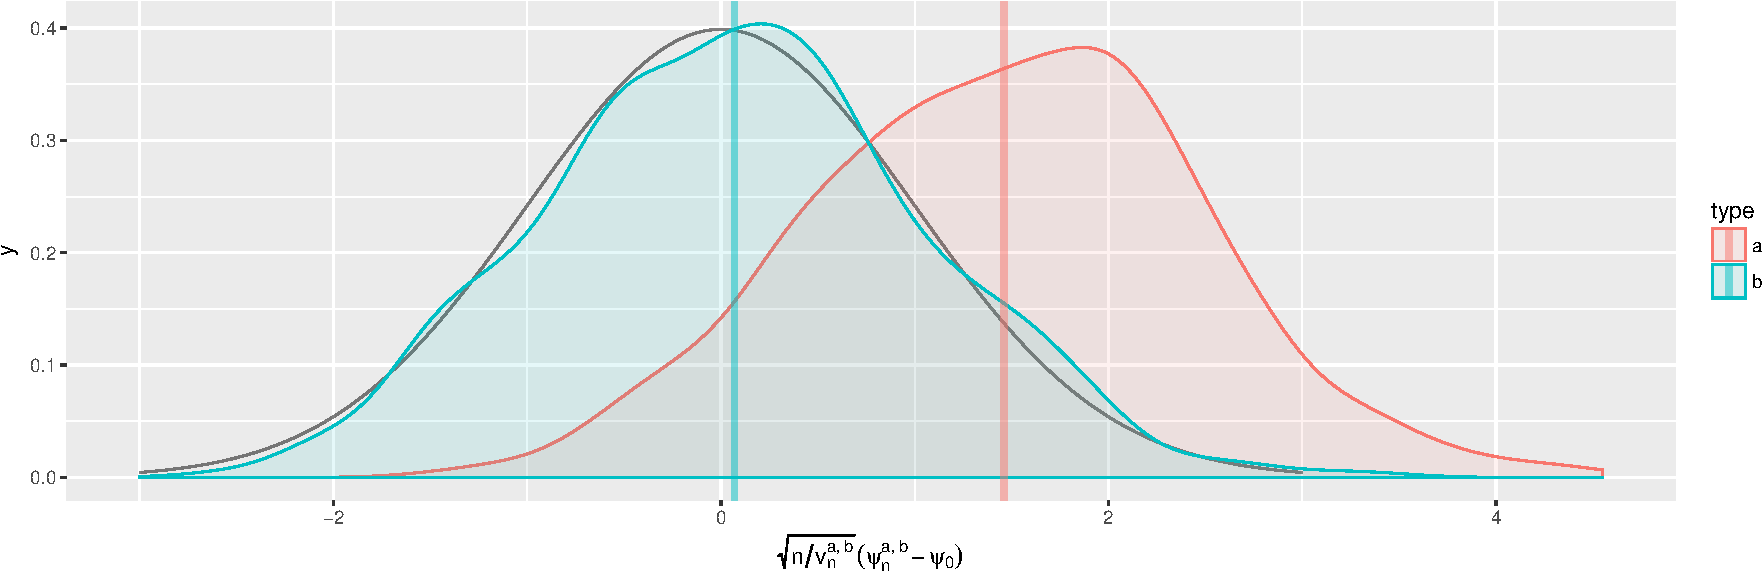
\includegraphics{img/known-Gbar-one-b-1.pdf}
\caption{\label{fig:known-Gbar-one-b}Kernel density estimators of the law of
two estimators of \(\psi_{0}\) (recentered with respect to \(\psi_{0}\),
and renormalized), one of them misconceived (a), the other assuming that
\(\Gbar_{0}\) is known (b). Built based on \texttt{iter} independent
realizations of each estimator.}
\end{figure}

Let \(v_{n}^{a}\) be \(n\) times the empirical variance of the
\texttt{iter} realizations of \(\psi_{n}^{a}\). By the above chunk of
code, the averages of \(\sqrt{n/v_{n}^{a}} (\psi_{n}^{a} - \psi_{0})\)
and \(\sqrt{n/v_{n}^{b}} (\psi_{n}^{b} - \psi_{0})\) computed across the
realizations of the two estimators are respectively equal to 1.461 and
0.07 (both rounded to three decimal places --- see \texttt{bias\_ab}).
Interpreted as amounts of bias, those two quantities are represented by
vertical lines in Figure \ref{fig:known-Gbar-one-b}. The red and blue
bell-shaped curves represent the empirical laws of \(\psi_{n}^{a}\) and
\(\psi_{n}^{b}\) (recentered with respect to \(\\psi_{0}\), and
renormalized) as estimated by kernel density estimation. The latter is
close to the black curve, which represents the standard normal density.

\subsection[Inference assuming $\Gbar_{0}$ known, or not, second pass.]{Inference assuming
$\boldsymbol{\Gbar_{0}}$ known, or not, second pass.} 
\label{subsec:known:gbar:two}

At the beginning of Section \ref{subsec:known:gbar:one}, we assumed that
\(\Gbar_{0}\) was known. Let us suppose now that it is not. The
definition of \(\psi_{n}^{b}\) can be adapted to overcome this
difficulty, by substituting an estimator of \(\ell\Gbar_{0}\) for
\(\ell\Gbar_{0}\) in \eqref{eq:psi:n:b}.

For simplicity, we consider the case that \(\Gbar_{0}\) is estimated by
minimizing a loss function on a single working model, both
fine-tune-parameter-free. By adopting this stance, we exclude estimating
procedures that involve penalization (\textit{e.g.} the LASSO) or
aggregation of competing estimators (\textit{via} stacking/super
learning) -- see Section \ref{subsec:exo:one}. Defined in the next chunk
of code, the generic function \texttt{estimate\_G} fits a user-specified
working model by minimizing the empirical risk associated to the
user-specified loss function and provided data.

\tcg{Comment on new structure of} \texttt{estimate\_G}
\tcg{and say a few words about} \texttt{compute\_lGhatAW}.

\begin{Shaded}
\begin{Highlighting}[]
\NormalTok{estimate_G <-}\StringTok{ }\ControlFlowTok{function}\NormalTok{(dat, algorithm, ...) \{}
  \ControlFlowTok{if}\NormalTok{ (}\OperatorTok{!}\KeywordTok{attr}\NormalTok{(algorithm, }\StringTok{"ML"}\NormalTok{)) \{}
\NormalTok{    dat <-}\StringTok{ }\KeywordTok{as.data.frame}\NormalTok{(dat)}
\NormalTok{    fit <-}\StringTok{ }\NormalTok{algorithm[[}\DecValTok{1}\NormalTok{]](}\DataTypeTok{formula =}\NormalTok{ algorithm[[}\DecValTok{2}\NormalTok{]], }\DataTypeTok{data =}\NormalTok{ dat)}
\NormalTok{    Ghat <-}\StringTok{ }\ControlFlowTok{function}\NormalTok{(newdata) \{}
\NormalTok{      newdata <-}\StringTok{ }\KeywordTok{as.data.frame}\NormalTok{(newdata)}
      \KeywordTok{predict}\NormalTok{(fit, newdata, }\DataTypeTok{type =} \StringTok{"response"}\NormalTok{)}
\NormalTok{    \}}
\NormalTok{  \} }\ControlFlowTok{else}\NormalTok{ \{}
\NormalTok{    fit <-}\StringTok{ }\KeywordTok{algorithm}\NormalTok{(dat, ...)}
\NormalTok{    Qhat <-}\StringTok{ }\ControlFlowTok{function}\NormalTok{(newdata) \{}
\NormalTok{      caret}\OperatorTok{::}\KeywordTok{predict.train}\NormalTok{(fit, newdata)}
\NormalTok{    \}}
\NormalTok{  \}}
  \KeywordTok{return}\NormalTok{(Ghat)}
\NormalTok{\}}

\NormalTok{compute_lGhatAW <-}\StringTok{ }\ControlFlowTok{function}\NormalTok{(A, W, Ghat, }\DataTypeTok{threshold =} \FloatTok{0.05}\NormalTok{) \{}
\NormalTok{  dat <-}\StringTok{ }\KeywordTok{data.frame}\NormalTok{(}\DataTypeTok{A =}\NormalTok{ A, }\DataTypeTok{W =}\NormalTok{ W)}
\NormalTok{  Ghat_W <-}\StringTok{ }\KeywordTok{Ghat}\NormalTok{(dat)}
\NormalTok{  lGAW <-}\StringTok{ }\NormalTok{A }\OperatorTok{*}\StringTok{ }\NormalTok{Ghat_W }\OperatorTok{+}\StringTok{ }\NormalTok{(}\DecValTok{1} \OperatorTok{-}\StringTok{ }\NormalTok{A) }\OperatorTok{*}\StringTok{ }\NormalTok{(}\DecValTok{1} \OperatorTok{-}\StringTok{ }\NormalTok{Ghat_W)}
\NormalTok{  pred <-}\StringTok{ }\KeywordTok{pmin}\NormalTok{(}\DecValTok{1} \OperatorTok{-}\StringTok{ }\NormalTok{threshold, }\KeywordTok{pmax}\NormalTok{(lGAW, threshold))}
  \KeywordTok{return}\NormalTok{(pred)}
\NormalTok{\}}
\end{Highlighting}
\end{Shaded}

Note how the prediction of any \(\ell\Gbar_{0}(A,W)\) is manually
bounded away from 0 and 1 at the last but one line of
\texttt{compute\_lGhatAW}. This is desirable because the
\textit{inverse} of each \(\ell\Gbar_{0}(A_{i},W_{i})\) appears in the
definition of \(\psi_{n}^{b}\) \eqref{eq:psi:n:b}.

For sake of illustration, we choose argument
\texttt{working\_model\_G\_one} of function \texttt{estimate\_G} as
follows:

\begin{Shaded}
\begin{Highlighting}[]
\NormalTok{working_model_G_one <-}\StringTok{ }\KeywordTok{list}\NormalTok{(}
  \DataTypeTok{model =} \ControlFlowTok{function}\NormalTok{(...) \{}\KeywordTok{glm}\NormalTok{(}\DataTypeTok{family =} \KeywordTok{binomial}\NormalTok{(), ...)\},}
  \DataTypeTok{formula =} \KeywordTok{as.formula}\NormalTok{(}
    \KeywordTok{paste}\NormalTok{(}\StringTok{"A ~"}\NormalTok{,}
          \KeywordTok{paste}\NormalTok{(}\KeywordTok{c}\NormalTok{(}\StringTok{"I(W^"}\NormalTok{, }\StringTok{"I(abs(W - 5/12)^"}\NormalTok{),}
                \KeywordTok{rep}\NormalTok{(}\KeywordTok{seq}\NormalTok{(}\DecValTok{1}\OperatorTok{/}\DecValTok{2}\NormalTok{, }\DecValTok{3}\OperatorTok{/}\DecValTok{2}\NormalTok{, }\DataTypeTok{by =} \DecValTok{1}\OperatorTok{/}\DecValTok{2}\NormalTok{), }\DataTypeTok{each =} \DecValTok{2}\NormalTok{),}
                \DataTypeTok{sep =} \StringTok{""}\NormalTok{, }\DataTypeTok{collapse =} \StringTok{") + "}\NormalTok{),}
          \StringTok{")"}\NormalTok{)}
\NormalTok{  ))}
\KeywordTok{attr}\NormalTok{(working_model_G_one, }\StringTok{"ML"}\NormalTok{) <-}\StringTok{ }\OtherTok{FALSE}
\NormalTok{working_model_G_one}\OperatorTok{$}\NormalTok{formula}
\end{Highlighting}
\end{Shaded}

\begin{verbatim}
## A ~ I(W^0.5) + I(abs(W - 5/12)^0.5) + I(W^1) + I(abs(W - 5/12)^1) + 
##     I(W^1.5) + I(abs(W - 5/12)^1.5)
\end{verbatim}

In words, we choose the so called logistic (or negative binomial) loss
function \(L_{a}\) given by \begin{equation}    \label{eq:logis:loss}
-L_{a}(f)(A,W) \equiv A \log f(W) + (1 - A) \log (1 - f(W)) \end{equation}
for any function \(f : [0,1] \to [0,1]\) paired with the working model
\(\calF \equiv \left\{f_{\theta} : \theta \in \bbR^{5}\right\}\) where,
for any \(\theta \in \bbR^{5}\),
\(\logit f_{\theta} (W) \equiv \theta_{0} + \sum_{j=1}^{4} \theta_{j} W^{j/2}\).
The working model is well specified: it happens that \(\Gbar_{0}\) is
the unique minimizer of the risk entailed by \(L_{a}\) over \(\calF\):
\begin{equation*}\Gbar_{0} = \mathop{\arg\min}_{f_{\theta} \in \calF}
\Exp_{P_{0}}   \left(L_{a}(f_{\theta})(A,W)\right).\end{equation*}
Therefore, the estimator \(\Gbar_{n}\) output by \texttt{estimate\_G}
and obtained by minimizing the empirical risk
\begin{equation*}        \Exp_{P_{n}}
\left(L_{a}(f_{\theta})(A,W)\right)      =     \frac{1}{n}      \sum_{i=1}^{n}
L_{a}(f_{\theta})(A_{i},W_{i})\end{equation*} over \(\calF\)
consistently estimates \(\Gbar_{0}\).

In light of \eqref{eq:psi:n:b}, introduce
\begin{equation}\psi_{n}^{c} \equiv
\frac{1}{n}   \sum_{i=1}^{n}   \left(\frac{2A_{i}  -   1}{\ell\Gbar_{n}(A_{i},
W_{i})}   Y_{i}\right).\end{equation} Because \(\Gbar_{n}\) minimizes
the empirical risk over a finite-dimensional and well-specified working
model, \(\sqrt{n} (\psi_{n}^{c} - \psi_{0})\) converges in law to a
centered Gaussian law. Let us compute \(\psi_{n}^{c}\) on the same
\texttt{iter\ =} 1000 independent samples of independent observations
drawn from \(P_{0}\) as in Section \ref{subsec:known:gbar:one}:

\begin{Shaded}
\begin{Highlighting}[]
\NormalTok{learned_features_fixed_sample_size <-}
\StringTok{  }\NormalTok{obs }\OperatorTok\StringTok{ }\KeywordTok{as_tibble}\NormalTok{() }\OperatorTok
\StringTok{  }\KeywordTok{mutate}\NormalTok{(}\DataTypeTok{id =} \DecValTok{1}\OperatorTok{:}\KeywordTok{n}\NormalTok{() }\OperatorTok\StringTok{ }\NormalTok{iter) }\OperatorTok
\StringTok{  }\KeywordTok{nest}\NormalTok{(}\OperatorTok{-}\NormalTok{id, }\DataTypeTok{.key =} \StringTok{"obs"}\NormalTok{) }\OperatorTok
\StringTok{  }\KeywordTok{mutate}\NormalTok{(}\DataTypeTok{Ghat =} \KeywordTok{map}\NormalTok{(obs, }\OperatorTok{~}\StringTok{ }\KeywordTok{estimate_G}\NormalTok{(., }\DataTypeTok{algorithm =}\NormalTok{ working_model_G_one))) }\OperatorTok
\StringTok{  }\KeywordTok{mutate}\NormalTok{(}\DataTypeTok{lGAW =} \KeywordTok{map2}\NormalTok{(Ghat, obs, }\OperatorTok{~}\StringTok{ }\KeywordTok{compute_lGhatAW}\NormalTok{(.y}\OperatorTok{$}\NormalTok{A, .y}\OperatorTok{$}\NormalTok{W, .x)))}


\NormalTok{psi_hat_abc <-}
\StringTok{  }\NormalTok{learned_features_fixed_sample_size }\OperatorTok
\StringTok{  }\KeywordTok{unnest}\NormalTok{(obs, lGAW) }\OperatorTok
\StringTok{  }\KeywordTok{group_by}\NormalTok{(id) }\OperatorTok
\StringTok{  }\KeywordTok{summarize}\NormalTok{(}\DataTypeTok{est =} \KeywordTok{mean}\NormalTok{(Y }\OperatorTok{*}\StringTok{ }\NormalTok{(}\DecValTok{2} \OperatorTok{*}\StringTok{ }\NormalTok{A }\OperatorTok{-}\StringTok{ }\DecValTok{1}\NormalTok{) }\OperatorTok{/}\StringTok{ }\NormalTok{lGAW)) }\OperatorTok
\StringTok{  }\KeywordTok{mutate}\NormalTok{(}\DataTypeTok{std =} \KeywordTok{sd}\NormalTok{(est),}
         \DataTypeTok{clt =}\NormalTok{ (est }\OperatorTok{-}\StringTok{ }\NormalTok{psi_approx) }\OperatorTok{/}\StringTok{ }\NormalTok{std,}
         \DataTypeTok{type =} \StringTok{"c"}\NormalTok{) }\OperatorTok
\StringTok{  }\KeywordTok{full_join}\NormalTok{(psi_hat_ab)}

\NormalTok{(bias_abc <-}\StringTok{ }\NormalTok{psi_hat_abc }\OperatorTok\StringTok{ }\KeywordTok{group_by}\NormalTok{(type) }\OperatorTok\StringTok{ }\KeywordTok{summarise}\NormalTok{(}\DataTypeTok{bias =} \KeywordTok{mean}\NormalTok{(clt)))}
\end{Highlighting}
\end{Shaded}

\begin{verbatim}
## # A tibble: 3 x 2
##   type    bias
##   <chr>  <dbl>
## 1 a     1.46  
## 2 b     0.0696
## 3 c     0.0435
\end{verbatim}

Note how we exploit the independent realizations of \(\psi_{n}^{c}\) to
estimate the asymptotic variance of the estimator with \(v_{n}^{c}/n\).
By the above chunk of code, the average of
\(\sqrt{n/v_{n}^{c}} (\psi_{n}^{c} - \psi_{0})\) computed across the
realizations is equal to 0.043 (rounded to three decimal places --- see
\texttt{bias\_abc}). We represent the empirical laws of the recentered
(with respect to \(\\psi_{0}\)) and renormalized \(\psi_{n}^{a}\),
\(\psi_{n}^{b}\) and \(\psi_{n}^{c}\) in Figures
\ref{fig:unknown-Gbar-three} (kernel density estimators) and
\ref{fig:unknown-Gbar-four} (quantile-quantile plots).

\begin{Shaded}
\begin{Highlighting}[]
\NormalTok{fig }\OperatorTok{+}
\StringTok{  }\KeywordTok{geom_density}\NormalTok{(}\KeywordTok{aes}\NormalTok{(clt, }\DataTypeTok{fill =}\NormalTok{ type, }\DataTypeTok{colour =}\NormalTok{ type), psi_hat_abc, }\DataTypeTok{alpha =} \FloatTok{0.1}\NormalTok{) }\OperatorTok{+}
\StringTok{  }\KeywordTok{geom_vline}\NormalTok{(}\KeywordTok{aes}\NormalTok{(}\DataTypeTok{xintercept =}\NormalTok{ bias, }\DataTypeTok{colour =}\NormalTok{ type),}
\NormalTok{             bias_abc, }\DataTypeTok{size =} \FloatTok{1.5}\NormalTok{, }\DataTypeTok{alpha =} \FloatTok{0.5}\NormalTok{) }\OperatorTok{+}
\StringTok{  }\KeywordTok{xlim}\NormalTok{(}\OperatorTok{-}\DecValTok{3}\NormalTok{, }\DecValTok{4}\NormalTok{) }\OperatorTok{+}\StringTok{ }
\StringTok{  }\KeywordTok{labs}\NormalTok{(}\DataTypeTok{x =} \KeywordTok{expression}\NormalTok{(}\KeywordTok{paste}\NormalTok{(}\KeywordTok{sqrt}\NormalTok{(n}\OperatorTok{/}\NormalTok{v[n]}\OperatorTok{^}\NormalTok{\{}\KeywordTok{list}\NormalTok{(a, b, c)\})}\OperatorTok{*}
\StringTok{                            }\NormalTok{(psi[n]}\OperatorTok{^}\NormalTok{\{}\KeywordTok{list}\NormalTok{(a, b, c)\} }\OperatorTok{-}\StringTok{ }\NormalTok{psi[}\DecValTok{0}\NormalTok{]))))}
\end{Highlighting}
\end{Shaded}

\begin{figure}
\centering
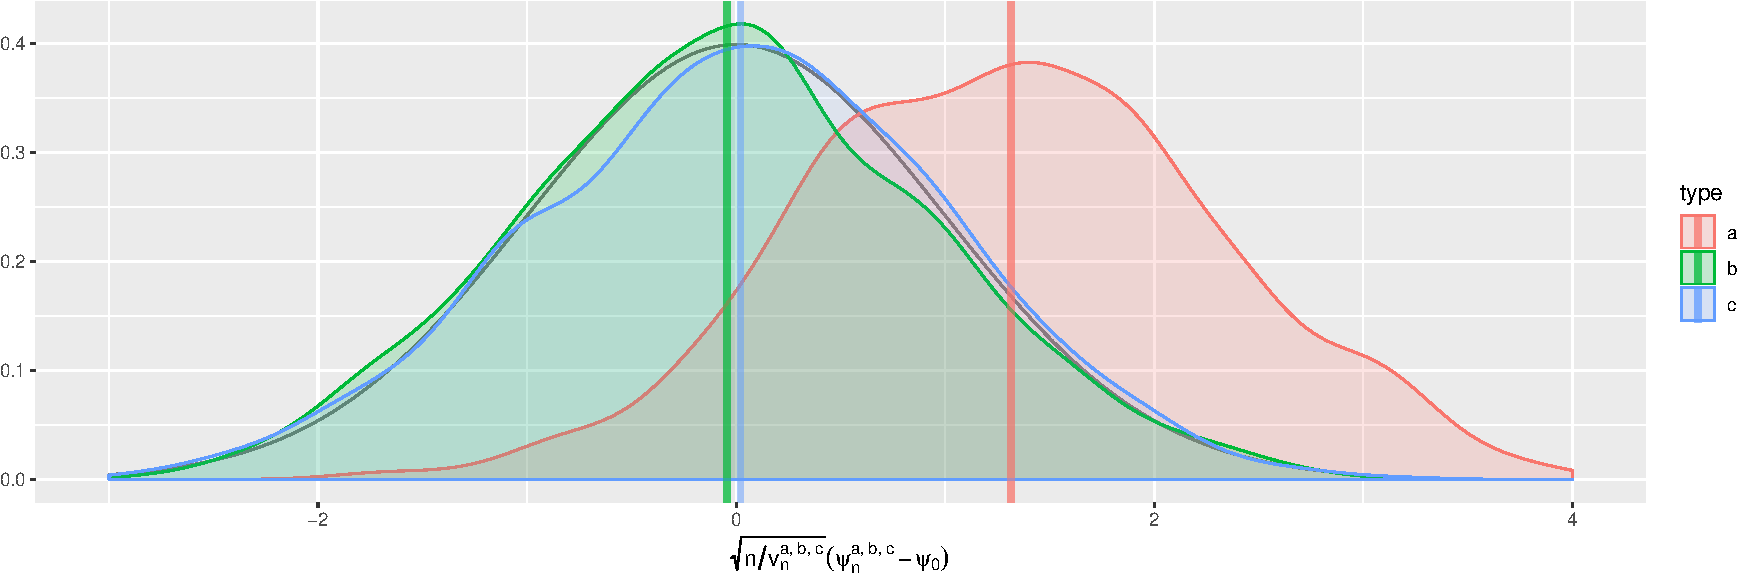
\includegraphics{img/unknown-Gbar-three-1.pdf}
\caption{\label{fig:unknown-Gbar-three}Kernel density estimators of the law
of three estimators of \(\psi_{0}\) (recentered with respect to
\(\psi_{0}\), and renormalized), one of them misconceived (a), one
assuming that \(\Gbar_{0}\) is known (b) and one that hinges on the
estimation of \(\Gbar_{0}\) (c). The present figure includes Figure
\ref{fig:known-Gbar-one-b} (but the colors differ). Built based on
\texttt{iter} independent realizations of each estimator.}
\end{figure}

\begin{Shaded}
\begin{Highlighting}[]
\KeywordTok{ggplot}\NormalTok{(psi_hat_abc, }\KeywordTok{aes}\NormalTok{(}\DataTypeTok{sample =}\NormalTok{ clt, }\DataTypeTok{fill =}\NormalTok{ type, }\DataTypeTok{colour =}\NormalTok{ type)) }\OperatorTok{+}
\StringTok{  }\KeywordTok{geom_abline}\NormalTok{(}\DataTypeTok{intercept =} \DecValTok{0}\NormalTok{, }\DataTypeTok{slope =} \DecValTok{1}\NormalTok{, }\DataTypeTok{alpha =} \FloatTok{0.5}\NormalTok{) }\OperatorTok{+}
\StringTok{  }\KeywordTok{geom_qq}\NormalTok{(}\DataTypeTok{alpha =} \DecValTok{1}\NormalTok{)}
\end{Highlighting}
\end{Shaded}

\begin{figure}
\centering
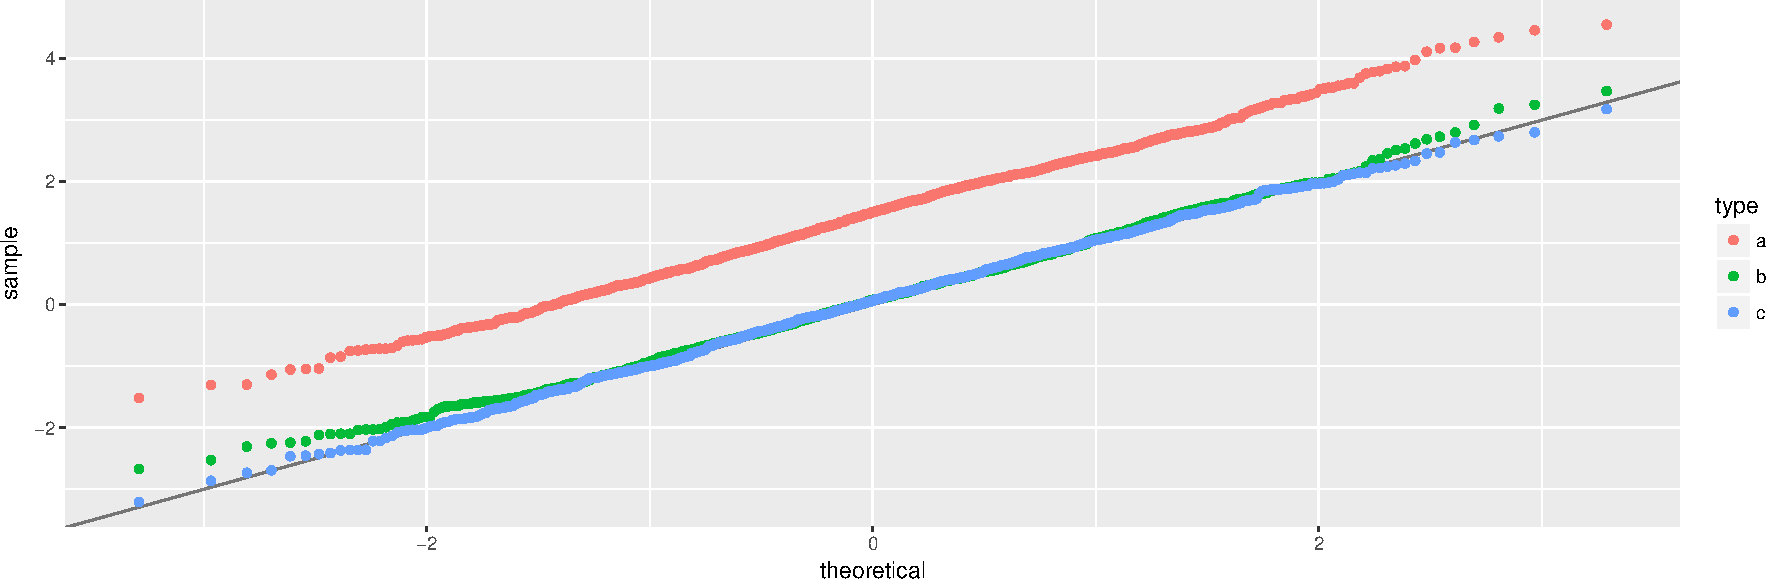
\includegraphics{img/unknown-Gbar-four-1.pdf}
\caption{\label{fig:unknown-Gbar-four}Quantile-quantile plot of the standard
normal law against the empirical laws of three estimators of
\(\psi_{0}\), one of them misconceived (a), one assuming that
\(\Gbar_{0}\) is known (b) and one that hinges on the estimation of
\(\Gbar_{0}\) (c). Built based on \texttt{iter} independent realizations
of each estimator.}
\end{figure}

Figures \ref{fig:unknown-Gbar-three} and \ref{fig:unknown-Gbar-four}
reveal that \(\psi_{n}^{c}\) behaves as well as \(\psi_{n}^{b}\) --- but
remember that we did not discuss how to estimate its asymptotic
variance.

\subsection{\gear Exercises.}
\label{subsec:exo:one}

The problems come within the context of Sections
\ref{subsec:known:gbar:one} and \ref{subsec:known:gbar:two}.

\begin{enumerate}
\def\labelenumi{\arabic{enumi}.}
\item
  Compute a numerical approximation of
  \(\Exp_{P_{0}} (Y | A=1) - \Exp_{P_{0}} (Y | A=0)\). How accurate is
  it?
\item
  Building upon the piece of code devoted to the repeated computation of
  \(\psi_{n}^{b}\) and its companion quantities, construct confidence
  intervals for \(\psi_{0}\) of (asymptotic) level \(95\%\), and check
  if the empirical coverage is satisfactory. Note that if the coverage
  was exactly \(95\%\), then the number of confidence intervals that
  would contain \(\psi_{0}\) would follow a binomial law with parameters
  \texttt{iter} and \texttt{0.95}, and recall that function
  \texttt{binom.test} performs an exact test of a simple null hypothesis
  about the probability of success in a Bernoulli experiment against its
  three one-sided and two-sided alternatives.
\item
  The call to \texttt{compute\_lGhatAW} makes predictions on the same
  data points as those exploited to learn \(\Gbar_{0}\) by fitting the
  user-supplied working model. Why could that be problematic? Can you
  think of a simple workaround, implement and test it?
\item
  Discuss what happens when the dimension of the (still well-specified)
  working model grows. You could use the following chunk of code
\end{enumerate}

\begin{Shaded}
\begin{Highlighting}[]
\NormalTok{powers <-}\StringTok{ }\NormalTok{## make sure '1/2' and '1' belong to 'powers', eg}
\StringTok{  }\KeywordTok{seq}\NormalTok{(}\DecValTok{1}\OperatorTok{/}\DecValTok{4}\NormalTok{, }\DecValTok{3}\NormalTok{, }\DataTypeTok{by =} \DecValTok{1}\OperatorTok{/}\DecValTok{4}\NormalTok{)}
\NormalTok{working_model_G_two <-}\StringTok{ }\KeywordTok{list}\NormalTok{(}
  \DataTypeTok{model =} \ControlFlowTok{function}\NormalTok{(...) \{}\KeywordTok{glm}\NormalTok{(}\DataTypeTok{family =} \KeywordTok{binomial}\NormalTok{(), ...)\},}
  \DataTypeTok{formula =} \KeywordTok{as.formula}\NormalTok{(}
    \KeywordTok{paste}\NormalTok{(}\StringTok{"A ~"}\NormalTok{,}
          \KeywordTok{paste}\NormalTok{(}\KeywordTok{c}\NormalTok{(}\StringTok{"I(W^"}\NormalTok{, }\StringTok{"I(abs(W - 5/12)^"}\NormalTok{),}
                \KeywordTok{rep}\NormalTok{(powers, }\DataTypeTok{each =} \DecValTok{2}\NormalTok{),}
                \DataTypeTok{sep =} \StringTok{""}\NormalTok{, }\DataTypeTok{collapse =} \StringTok{") + "}\NormalTok{),}
          \StringTok{")"}\NormalTok{)}
\NormalTok{  ))}
\KeywordTok{attr}\NormalTok{(working_model_G_two, }\StringTok{"ML"}\NormalTok{) <-}\StringTok{ }\OtherTok{FALSE}
\end{Highlighting}
\end{Shaded}

play around with argument \texttt{powers} (making sure that \texttt{1/2}
and \texttt{1} belong to it), and plot graphics similar to those
presented in Figures \ref{fig:unknown-Gbar-three} and
\ref{fig:unknown-Gbar-four}.

\begin{enumerate}
\def\labelenumi{\arabic{enumi}.}
\setcounter{enumi}{4}
\tightlist
\item
  Discuss what happens when the working model is mis-specified. You
  could use the following chunk of code:
\end{enumerate}

\begin{Shaded}
\begin{Highlighting}[]
\NormalTok{transform <-}\StringTok{ }\KeywordTok{c}\NormalTok{(}\StringTok{"cos"}\NormalTok{, }\StringTok{"sin"}\NormalTok{, }\StringTok{"sqrt"}\NormalTok{, }\StringTok{"log"}\NormalTok{, }\StringTok{"exp"}\NormalTok{)}
\NormalTok{working_model_G_three <-}\StringTok{ }\KeywordTok{list}\NormalTok{(}
  \DataTypeTok{model =} \ControlFlowTok{function}\NormalTok{(...) \{}\KeywordTok{glm}\NormalTok{(}\DataTypeTok{family =} \KeywordTok{binomial}\NormalTok{(), ...)\},}
  \DataTypeTok{formula =} \KeywordTok{as.formula}\NormalTok{(}
    \KeywordTok{paste}\NormalTok{(}\StringTok{"A ~"}\NormalTok{,}
          \KeywordTok{paste}\NormalTok{(}\StringTok{"I("}\NormalTok{, transform, }\DataTypeTok{sep =} \StringTok{""}\NormalTok{, }\DataTypeTok{collapse =} \StringTok{"(W)) + "}\NormalTok{),}
          \StringTok{"(W))"}\NormalTok{)}
\NormalTok{  ))}
\KeywordTok{attr}\NormalTok{(working_model_G_three, }\StringTok{"ML"}\NormalTok{) <-}\StringTok{ }\OtherTok{FALSE}
\NormalTok{(working_model_G_three}\OperatorTok{$}\NormalTok{formula)}
\end{Highlighting}
\end{Shaded}

\begin{verbatim}
## A ~ I(cos(W)) + I(sin(W)) + I(sqrt(W)) + I(log(W)) + I(exp(W))
\end{verbatim}

\begin{enumerate}
\def\labelenumi{\arabic{enumi}.}
\setcounter{enumi}{5}
\tightlist
\item
  \textdbend  Drawing inspiration from \eqref{eq:v:n:b}, one may
  consider estimating the asymptotic variance of \(\psi_{n}^{c}\) with
  the counterpart of \(v_{n}^{b}\) obtained by substituting
  \(\ell\Gbar_{n}\) for \(\ell\Gbar_{0}\) in \eqref{eq:v:n:b}. By
  adapting the piece of code devoted to the repeated computation of
  \(\psi_{n}^{b}\) and its companion quantities, discuss if that would
  be legitimate.
\end{enumerate}

\subsection[Inference based on the estimation of $\Qbar_{0}$.]{Inference based
on the estimation of $\boldsymbol{\Qbar_{0}}$.} 
\label{subsec:inf:Q0}

\tcg{Comment on structure of} \texttt{estimate\_Q}, similar to that of
\texttt{estimate\_G}.

\tcg{Demonstrating the  inference of} \(\psi_{0}\)
\tcg{based  on the estimation
of} \(\Qbar_{0}\) \tcg{(and of the marginal  law of}
\(W\)\tcg{).  Once based on a
(mis-specified) working model, and once based on a non-parametric algorithm.}

\begin{Shaded}
\begin{Highlighting}[]
\NormalTok{estimate_Q <-}\StringTok{ }\ControlFlowTok{function}\NormalTok{(dat, algorithm, ...) \{}
  \ControlFlowTok{if}\NormalTok{ (}\OperatorTok{!}\KeywordTok{attr}\NormalTok{(algorithm, }\StringTok{"ML"}\NormalTok{)) \{}
\NormalTok{    dat <-}\StringTok{ }\KeywordTok{as.data.frame}\NormalTok{(dat)}
\NormalTok{    fit <-}\StringTok{ }\NormalTok{algorithm[[}\DecValTok{1}\NormalTok{]](}\DataTypeTok{formula =}\NormalTok{ algorithm[[}\DecValTok{2}\NormalTok{]], }\DataTypeTok{data =}\NormalTok{ dat)}
\NormalTok{    Qhat <-}\StringTok{ }\ControlFlowTok{function}\NormalTok{(newdata) \{}
\NormalTok{      newdata <-}\StringTok{ }\KeywordTok{as.data.frame}\NormalTok{(newdata)}
      \KeywordTok{predict}\NormalTok{(fit, newdata, }\DataTypeTok{type =} \StringTok{"response"}\NormalTok{)}
\NormalTok{    \}}
\NormalTok{  \} }\ControlFlowTok{else}\NormalTok{ \{}
\NormalTok{    fit <-}\StringTok{ }\KeywordTok{algorithm}\NormalTok{(dat, ...)}
\NormalTok{    Qhat <-}\StringTok{ }\ControlFlowTok{function}\NormalTok{(newdata) \{}
\NormalTok{      caret}\OperatorTok{::}\KeywordTok{predict.train}\NormalTok{(fit, newdata)}
\NormalTok{    \}    }
\NormalTok{  \}}
  \KeywordTok{return}\NormalTok{(Qhat)}
\NormalTok{\}}

\NormalTok{compute_QhatAW <-}\StringTok{ }\ControlFlowTok{function}\NormalTok{(Y, A, W, Qhat, }\DataTypeTok{blip =} \OtherTok{FALSE}\NormalTok{) \{}
  \ControlFlowTok{if}\NormalTok{ (}\OperatorTok{!}\NormalTok{blip) \{}
\NormalTok{    dat <-}\StringTok{ }\KeywordTok{data.frame}\NormalTok{(}\DataTypeTok{Y =}\NormalTok{ Y, }\DataTypeTok{A =}\NormalTok{ A, }\DataTypeTok{W =}\NormalTok{ W)}
\NormalTok{    pred <-}\StringTok{ }\KeywordTok{Qhat}\NormalTok{(dat)}
\NormalTok{  \} }\ControlFlowTok{else}\NormalTok{ \{}
\NormalTok{    pred <-}\StringTok{ }\KeywordTok{Qhat}\NormalTok{(}\KeywordTok{data.frame}\NormalTok{(}\DataTypeTok{A =} \DecValTok{1}\NormalTok{, }\DataTypeTok{W =}\NormalTok{ W)) }\OperatorTok{-}\StringTok{ }\KeywordTok{Qhat}\NormalTok{(}\KeywordTok{data.frame}\NormalTok{(}\DataTypeTok{A =} \DecValTok{0}\NormalTok{, }\DataTypeTok{W =}\NormalTok{ W))}
\NormalTok{  \}}
  \KeywordTok{return}\NormalTok{(pred)  }
\NormalTok{\}}

\NormalTok{working_model_Q_one <-}\StringTok{ }\KeywordTok{list}\NormalTok{(}
  \DataTypeTok{model =} \ControlFlowTok{function}\NormalTok{(...) \{}\KeywordTok{glm}\NormalTok{(}\DataTypeTok{family =} \KeywordTok{binomial}\NormalTok{(), ...)\},}
  \DataTypeTok{formula =} \KeywordTok{as.formula}\NormalTok{(}
    \KeywordTok{paste}\NormalTok{(}\StringTok{"Y ~ A * ("}\NormalTok{,}
          \KeywordTok{paste}\NormalTok{(}\StringTok{"I(W^"}\NormalTok{, }\KeywordTok{seq}\NormalTok{(}\DecValTok{1}\OperatorTok{/}\DecValTok{2}\NormalTok{, }\DecValTok{3}\OperatorTok{/}\DecValTok{2}\NormalTok{, }\DataTypeTok{by =} \DecValTok{1}\OperatorTok{/}\DecValTok{2}\NormalTok{), }\DataTypeTok{sep =} \StringTok{""}\NormalTok{, }\DataTypeTok{collapse =} \StringTok{") + "}\NormalTok{),}
          \StringTok{"))"}\NormalTok{)}
\NormalTok{  ))}
\KeywordTok{attr}\NormalTok{(working_model_Q_one, }\StringTok{"ML"}\NormalTok{) <-}\StringTok{ }\OtherTok{FALSE}
\NormalTok{working_model_Q_one}\OperatorTok{$}\NormalTok{formula}
\end{Highlighting}
\end{Shaded}

\begin{verbatim}
## Y ~ A * (I(W^0.5) + I(W^1) + I(W^1.5))
\end{verbatim}

\begin{Shaded}
\begin{Highlighting}[]
\NormalTok{## k-NN}
\NormalTok{kknn_algo <-}\StringTok{ }\ControlFlowTok{function}\NormalTok{(dat, ...) \{}
\NormalTok{  args <-}\StringTok{ }\KeywordTok{list}\NormalTok{(...)}
  \ControlFlowTok{if}\NormalTok{ (}\StringTok{"Subsample"} \OperatorTok\StringTok{ }\KeywordTok{names}\NormalTok{(args)) \{}
\NormalTok{    keep <-}\StringTok{ }\KeywordTok{sample.int}\NormalTok{(}\KeywordTok{nrow}\NormalTok{(dat), args}\OperatorTok{$}\NormalTok{Subsample)}
\NormalTok{    dat <-}\StringTok{ }\NormalTok{dat[keep, ]}
\NormalTok{  \}}
\NormalTok{  caret}\OperatorTok{::}\KeywordTok{train}\NormalTok{(Y }\OperatorTok{~}\StringTok{ }\KeywordTok{I}\NormalTok{(}\DecValTok{10}\OperatorTok{*}\NormalTok{A) }\OperatorTok{+}\StringTok{ }\NormalTok{W, ## a tweak}
               \DataTypeTok{data =}\NormalTok{ dat,}
               \DataTypeTok{method =} \StringTok{"kknn"}\NormalTok{,}
               \DataTypeTok{verbose =} \OtherTok{FALSE}\NormalTok{,}
\NormalTok{               ...)}
\NormalTok{\}}
\KeywordTok{attr}\NormalTok{(kknn_algo, }\StringTok{"ML"}\NormalTok{) <-}\StringTok{ }\OtherTok{TRUE}
\NormalTok{kknn_grid <-}\StringTok{ }\KeywordTok{expand.grid}\NormalTok{(}\DataTypeTok{kmax =} \DecValTok{5}\NormalTok{, }\DataTypeTok{distance =} \DecValTok{2}\NormalTok{, }\DataTypeTok{kernel =} \StringTok{"gaussian"}\NormalTok{)}
\NormalTok{control <-}\StringTok{ }\KeywordTok{trainControl}\NormalTok{(}\DataTypeTok{method =} \StringTok{"cv"}\NormalTok{, }\DataTypeTok{number =} \DecValTok{2}\NormalTok{,}
                        \DataTypeTok{predictionBounds =} \KeywordTok{c}\NormalTok{(}\DecValTok{0}\NormalTok{, }\DecValTok{1}\NormalTok{),}
                        \DataTypeTok{allowParallel =} \OtherTok{TRUE}\NormalTok{)}
\end{Highlighting}
\end{Shaded}

\begin{Shaded}
\begin{Highlighting}[]
\NormalTok{learned_features_fixed_sample_size <-}
\StringTok{  }\NormalTok{learned_features_fixed_sample_size }\OperatorTok\StringTok{ }\CommentTok{# head(n = 100) %>%}
\StringTok{  }\KeywordTok{mutate}\NormalTok{(}\DataTypeTok{Qhat_d =} \KeywordTok{map}\NormalTok{(obs, }\OperatorTok{~}\StringTok{ }\KeywordTok{estimate_Q}\NormalTok{(., }\DataTypeTok{algorithm =}\NormalTok{ working_model_Q_one)),}
         \DataTypeTok{Qhat_e =} \KeywordTok{map}\NormalTok{(obs, }\OperatorTok{~}\StringTok{ }\KeywordTok{estimate_Q}\NormalTok{(., }\DataTypeTok{algorithm =}\NormalTok{ kknn_algo,}
                                        \DataTypeTok{trControl =}\NormalTok{ control,}
                                        \DataTypeTok{tuneGrid =}\NormalTok{ kknn_grid))) }\OperatorTok
\StringTok{  }\KeywordTok{mutate}\NormalTok{(}\DataTypeTok{blip_QW_d =} \KeywordTok{map2}\NormalTok{(Qhat_d, obs,}
                          \OperatorTok{~}\StringTok{ }\KeywordTok{compute_QhatAW}\NormalTok{(.y}\OperatorTok{$}\NormalTok{Y, .y}\OperatorTok{$}\NormalTok{A, .y}\OperatorTok{$}\NormalTok{W, .x, }\DataTypeTok{blip =} \OtherTok{TRUE}\NormalTok{)),}
         \DataTypeTok{blip_QW_e =} \KeywordTok{map2}\NormalTok{(Qhat_e, obs,}
                          \OperatorTok{~}\StringTok{ }\KeywordTok{compute_QhatAW}\NormalTok{(.y}\OperatorTok{$}\NormalTok{Y, .y}\OperatorTok{$}\NormalTok{A, .y}\OperatorTok{$}\NormalTok{W, .x, }\DataTypeTok{blip =} \OtherTok{TRUE}\NormalTok{)))}

\NormalTok{psi_hat_de <-}
\StringTok{  }\NormalTok{learned_features_fixed_sample_size }\OperatorTok
\StringTok{  }\KeywordTok{unnest}\NormalTok{(blip_QW_d, blip_QW_e) }\OperatorTok
\StringTok{  }\KeywordTok{group_by}\NormalTok{(id) }\OperatorTok
\StringTok{  }\KeywordTok{summarize}\NormalTok{(}\DataTypeTok{est_d =} \KeywordTok{mean}\NormalTok{(blip_QW_d),}
            \DataTypeTok{est_e =} \KeywordTok{mean}\NormalTok{(blip_QW_e)) }\OperatorTok
\StringTok{  }\KeywordTok{mutate}\NormalTok{(}\DataTypeTok{std_d =} \KeywordTok{sd}\NormalTok{(est_d),}
         \DataTypeTok{std_e =} \KeywordTok{sd}\NormalTok{(est_e),}
         \DataTypeTok{clt_d =}\NormalTok{ (est_d }\OperatorTok{-}\StringTok{ }\NormalTok{psi_approx) }\OperatorTok{/}\StringTok{ }\NormalTok{std_d,}
         \DataTypeTok{clt_e =}\NormalTok{ (est_e }\OperatorTok{-}\StringTok{ }\NormalTok{psi_approx) }\OperatorTok{/}\StringTok{ }\NormalTok{std_e) }\OperatorTok\StringTok{ }
\StringTok{  }\KeywordTok{gather}\NormalTok{(}\StringTok{"key"}\NormalTok{, }\StringTok{"value"}\NormalTok{, }\OperatorTok{-}\NormalTok{id) }\OperatorTok
\StringTok{  }\KeywordTok{extract}\NormalTok{(key, }\KeywordTok{c}\NormalTok{(}\StringTok{"what"}\NormalTok{, }\StringTok{"type"}\NormalTok{), }\StringTok{"([^_]+)_([de])"}\NormalTok{) }\OperatorTok
\StringTok{  }\KeywordTok{spread}\NormalTok{(what, value)}

\NormalTok{(bias_de <-}\StringTok{ }\NormalTok{psi_hat_de }\OperatorTok\StringTok{ }\KeywordTok{group_by}\NormalTok{(type) }\OperatorTok\StringTok{ }\KeywordTok{summarize}\NormalTok{(}\DataTypeTok{bias =} \KeywordTok{mean}\NormalTok{(clt)))}
\end{Highlighting}
\end{Shaded}

\begin{verbatim}
## # A tibble: 2 x 2
##   type    bias
##   <chr>  <dbl>
## 1 d     0.304 
## 2 e     0.0881
\end{verbatim}

\begin{Shaded}
\begin{Highlighting}[]
\NormalTok{fig <-}\StringTok{ }\KeywordTok{ggplot}\NormalTok{() }\OperatorTok{+}
\StringTok{  }\KeywordTok{geom_line}\NormalTok{(}\KeywordTok{aes}\NormalTok{(}\DataTypeTok{x =}\NormalTok{ x, }\DataTypeTok{y =}\NormalTok{ y), }
            \DataTypeTok{data =} \KeywordTok{tibble}\NormalTok{(}\DataTypeTok{x =} \KeywordTok{seq}\NormalTok{(}\OperatorTok{-}\DecValTok{3}\NormalTok{, }\DecValTok{3}\NormalTok{, }\DataTypeTok{length.out =} \FloatTok{1e3}\NormalTok{),}
                          \DataTypeTok{y =} \KeywordTok{dnorm}\NormalTok{(x)),}
            \DataTypeTok{linetype =} \DecValTok{1}\NormalTok{, }\DataTypeTok{alpha =} \FloatTok{0.5}\NormalTok{) }\OperatorTok{+}
\StringTok{  }\KeywordTok{geom_density}\NormalTok{(}\KeywordTok{aes}\NormalTok{(clt, }\DataTypeTok{fill =}\NormalTok{ type, }\DataTypeTok{colour =}\NormalTok{ type),}
\NormalTok{               psi_hat_de, }\DataTypeTok{alpha =} \FloatTok{0.1}\NormalTok{) }\OperatorTok{+}
\StringTok{  }\KeywordTok{geom_vline}\NormalTok{(}\KeywordTok{aes}\NormalTok{(}\DataTypeTok{xintercept =}\NormalTok{ bias, }\DataTypeTok{colour =}\NormalTok{ type),}
\NormalTok{             bias_de, }\DataTypeTok{size =} \FloatTok{1.5}\NormalTok{, }\DataTypeTok{alpha =} \FloatTok{0.5}\NormalTok{)}
  
\NormalTok{fig }\OperatorTok{+}
\StringTok{  }\KeywordTok{labs}\NormalTok{(}\DataTypeTok{x =} \KeywordTok{expression}\NormalTok{(}\KeywordTok{paste}\NormalTok{(}\KeywordTok{sqrt}\NormalTok{(n}\OperatorTok{/}\NormalTok{v[n]}\OperatorTok{^}\NormalTok{\{}\KeywordTok{list}\NormalTok{(d, e)\})}\OperatorTok{*}\NormalTok{(psi[n]}\OperatorTok{^}\NormalTok{\{}\KeywordTok{list}\NormalTok{(d, e)\} }\OperatorTok{-}\StringTok{ }\NormalTok{psi[}\DecValTok{0}\NormalTok{]))))}
\end{Highlighting}
\end{Shaded}

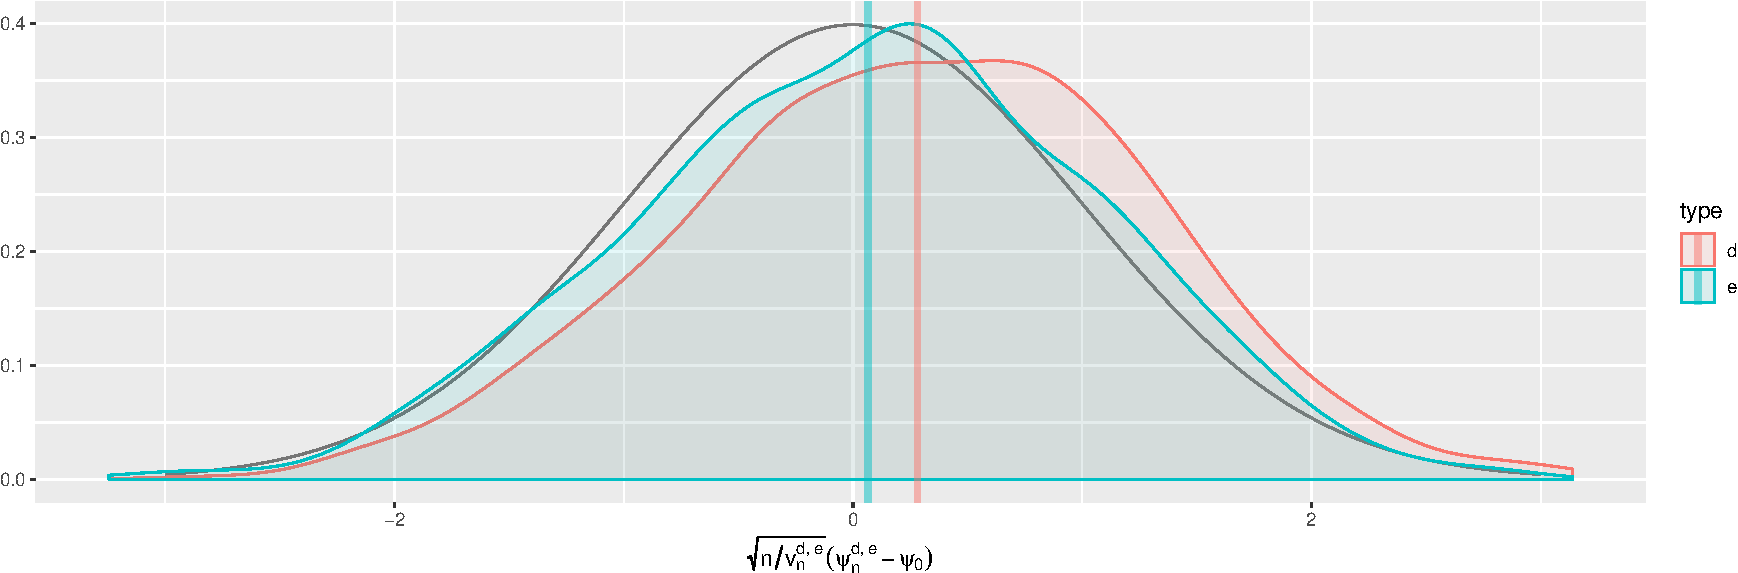
\includegraphics{img/estimating-Qbar-one-bis-1.pdf}

\tcg{No that bad!   Yet, we know that} \(\sqrt{n}\)
\tcg{times  bias is bound to
increase with sample size. To see this, check out the next chunks of code.}

\begin{Shaded}
\begin{Highlighting}[]
\NormalTok{sample_size <-}\StringTok{ }\KeywordTok{c}\NormalTok{(}\FloatTok{1e3}\NormalTok{, }\FloatTok{4e3}\NormalTok{, }\FloatTok{9e3}\NormalTok{)}
\NormalTok{block_size <-}\StringTok{ }\KeywordTok{sum}\NormalTok{(sample_size)}

\NormalTok{label <-}\StringTok{ }\ControlFlowTok{function}\NormalTok{(xx, }\DataTypeTok{sample_size =} \KeywordTok{c}\NormalTok{(}\FloatTok{1e3}\NormalTok{, }\FloatTok{2e3}\NormalTok{)) \{}
\NormalTok{  by <-}\StringTok{ }\KeywordTok{sum}\NormalTok{(sample_size)}
\NormalTok{  xx <-}\StringTok{ }\NormalTok{xx[}\KeywordTok{seq_len}\NormalTok{((}\KeywordTok{length}\NormalTok{(xx) }\OperatorTok\StringTok{ }\NormalTok{by) }\OperatorTok{*}\StringTok{ }\NormalTok{by)] }\OperatorTok{-}\StringTok{ }\DecValTok{1}
\NormalTok{  prefix <-}\StringTok{ }\NormalTok{xx }\OperatorTok\StringTok{ }\NormalTok{by}
\NormalTok{  suffix <-}\StringTok{ }\KeywordTok{findInterval}\NormalTok{(xx }\OperatorTok\StringTok{ }\NormalTok{by, }\KeywordTok{cumsum}\NormalTok{(sample_size))}
  \KeywordTok{paste}\NormalTok{(prefix }\OperatorTok{+}\StringTok{ }\DecValTok{1}\NormalTok{, suffix }\OperatorTok{+}\StringTok{ }\DecValTok{1}\NormalTok{, }\DataTypeTok{sep =} \StringTok{"_"}\NormalTok{)}
\NormalTok{\}}

\NormalTok{learned_features_varying_sample_size <-}\StringTok{ }\NormalTok{obs }\OperatorTok\StringTok{ }\NormalTok{as.tibble }\OperatorTok\StringTok{ }
\StringTok{  }\KeywordTok{head}\NormalTok{(}\DataTypeTok{n =}\NormalTok{ (}\KeywordTok{nrow}\NormalTok{(.) }\OperatorTok\StringTok{ }\NormalTok{block_size) }\OperatorTok{*}\StringTok{ }\NormalTok{block_size) }\OperatorTok\StringTok{ }
\StringTok{  }\KeywordTok{mutate}\NormalTok{(}\DataTypeTok{block =} \KeywordTok{label}\NormalTok{(}\DecValTok{1}\OperatorTok{:}\KeywordTok{nrow}\NormalTok{(.), sample_size)) }\OperatorTok
\StringTok{  }\KeywordTok{nest}\NormalTok{(}\OperatorTok{-}\NormalTok{block, }\DataTypeTok{.key =} \StringTok{"obs"}\NormalTok{)}
\end{Highlighting}
\end{Shaded}

First, we cut the data set into independent sub-data sets of sample size
\(n\) in \(\{\) 1000, 4000, 9000 \(\}\). Second, we infer \(\psi_{0}\)
as shown two chunks earlier. We thus obtain 71 independent realizations
of each estimator derived on data sets of 3, increasing sample sizes.

\begin{Shaded}
\begin{Highlighting}[]
\NormalTok{learned_features_varying_sample_size <-}
\StringTok{  }\NormalTok{learned_features_varying_sample_size }\OperatorTok\StringTok{ }
\StringTok{  }\KeywordTok{mutate}\NormalTok{(}\DataTypeTok{Qhat_d =} \KeywordTok{map}\NormalTok{(obs, }\OperatorTok{~}\StringTok{ }\KeywordTok{estimate_Q}\NormalTok{(., }\DataTypeTok{algorithm =}\NormalTok{ working_model_Q_one)),}
         \DataTypeTok{Qhat_e =} \KeywordTok{map}\NormalTok{(obs, }\OperatorTok{~}\StringTok{ }\KeywordTok{estimate_Q}\NormalTok{(., }\DataTypeTok{algorithm =}\NormalTok{ kknn_algo,}
                                        \DataTypeTok{trControl =}\NormalTok{ control,}
                                        \DataTypeTok{tuneGrid =}\NormalTok{ kknn_grid))) }\OperatorTok
\StringTok{  }\KeywordTok{mutate}\NormalTok{(}\DataTypeTok{blip_QW_d =} \KeywordTok{map2}\NormalTok{(Qhat_d, obs,}
                          \OperatorTok{~}\StringTok{ }\KeywordTok{compute_QhatAW}\NormalTok{(.y}\OperatorTok{$}\NormalTok{Y, .y}\OperatorTok{$}\NormalTok{A, .y}\OperatorTok{$}\NormalTok{W, .x, }\DataTypeTok{blip =} \OtherTok{TRUE}\NormalTok{)),}
         \DataTypeTok{blip_QW_e =} \KeywordTok{map2}\NormalTok{(Qhat_e, obs,}
                          \OperatorTok{~}\StringTok{ }\KeywordTok{compute_QhatAW}\NormalTok{(.y}\OperatorTok{$}\NormalTok{Y, .y}\OperatorTok{$}\NormalTok{A, .y}\OperatorTok{$}\NormalTok{W, .x, }\DataTypeTok{blip =} \OtherTok{TRUE}\NormalTok{)))}

\NormalTok{root_n_bias <-}\StringTok{ }\NormalTok{learned_features_varying_sample_size }\OperatorTok
\StringTok{  }\KeywordTok{unnest}\NormalTok{(blip_QW_d, blip_QW_e) }\OperatorTok
\StringTok{  }\KeywordTok{group_by}\NormalTok{(block) }\OperatorTok
\StringTok{  }\KeywordTok{summarize}\NormalTok{(}\DataTypeTok{clt_d =} \KeywordTok{sqrt}\NormalTok{(}\KeywordTok{n}\NormalTok{())}\OperatorTok{*}\NormalTok{(}\KeywordTok{mean}\NormalTok{(blip_QW_d) }\OperatorTok{-}\StringTok{ }\NormalTok{psi_approx),}
            \DataTypeTok{clt_e =} \KeywordTok{sqrt}\NormalTok{(}\KeywordTok{n}\NormalTok{())}\OperatorTok{*}\NormalTok{(}\KeywordTok{mean}\NormalTok{(blip_QW_e) }\OperatorTok{-}\StringTok{ }\NormalTok{psi_approx)) }\OperatorTok
\StringTok{  }\KeywordTok{gather}\NormalTok{(}\StringTok{"key"}\NormalTok{, }\StringTok{"value"}\NormalTok{, }\OperatorTok{-}\NormalTok{block) }\OperatorTok
\StringTok{  }\KeywordTok{extract}\NormalTok{(key, }\KeywordTok{c}\NormalTok{(}\StringTok{"what"}\NormalTok{, }\StringTok{"type"}\NormalTok{), }\StringTok{"([^_]+)_([de])"}\NormalTok{) }\OperatorTok
\StringTok{  }\KeywordTok{spread}\NormalTok{(what, value) }\OperatorTok
\StringTok{  }\KeywordTok{mutate}\NormalTok{(}\DataTypeTok{block =} \KeywordTok{unlist}\NormalTok{(}\KeywordTok{map}\NormalTok{(}\KeywordTok{strsplit}\NormalTok{(block, }\StringTok{"_"}\NormalTok{), }\OperatorTok{~}\NormalTok{.x[}\DecValTok{2}\NormalTok{])),}
         \DataTypeTok{sample_size =}\NormalTok{ sample_size[}\KeywordTok{as.integer}\NormalTok{(block)])}
\end{Highlighting}
\end{Shaded}

The \texttt{tibble} called \texttt{root\_n\_bias} reports root-\(n\)
times bias for all combinations of estimator and sample size. The next
chunk of code presents visually our findings. Note how we include the
realizations of the estimators derived earlier and contained in
\texttt{psi\_hat\_de} (thus breaking the independence between components
of \texttt{root\_n\_bias}, a small price to pay here).

\begin{Shaded}
\begin{Highlighting}[]
\NormalTok{root_n_bias <-}\StringTok{ }\NormalTok{learned_features_fixed_sample_size }\OperatorTok
\StringTok{  }\KeywordTok{mutate}\NormalTok{(}\DataTypeTok{sample_size =}\NormalTok{ B}\OperatorTok{/}\NormalTok{iter) }\OperatorTok\StringTok{  }\CommentTok{# because *fixed* sample size}
\StringTok{  }\KeywordTok{unnest}\NormalTok{(blip_QW_d, blip_QW_e) }\OperatorTok
\StringTok{  }\KeywordTok{group_by}\NormalTok{(id) }\OperatorTok
\StringTok{  }\KeywordTok{summarize}\NormalTok{(}\DataTypeTok{clt_d =} \KeywordTok{sqrt}\NormalTok{(}\KeywordTok{n}\NormalTok{()) }\OperatorTok{*}\StringTok{ }\NormalTok{(}\KeywordTok{mean}\NormalTok{(blip_QW_d) }\OperatorTok{-}\StringTok{ }\NormalTok{psi_approx),}
            \DataTypeTok{clt_e =} \KeywordTok{sqrt}\NormalTok{(}\KeywordTok{n}\NormalTok{()) }\OperatorTok{*}\StringTok{ }\NormalTok{(}\KeywordTok{mean}\NormalTok{(blip_QW_e) }\OperatorTok{-}\StringTok{ }\NormalTok{psi_approx),}
            \DataTypeTok{sample_size =}\NormalTok{ sample_size[}\DecValTok{1}\NormalTok{]) }\OperatorTok
\StringTok{  }\KeywordTok{gather}\NormalTok{(}\StringTok{"key"}\NormalTok{, }\StringTok{"clt"}\NormalTok{, }\OperatorTok{-}\NormalTok{id, }\OperatorTok{-}\NormalTok{sample_size) }\OperatorTok
\StringTok{  }\KeywordTok{extract}\NormalTok{(key, }\KeywordTok{c}\NormalTok{(}\StringTok{"what"}\NormalTok{, }\StringTok{"type"}\NormalTok{), }\StringTok{"([^_]+)_([de])"}\NormalTok{) }\OperatorTok
\StringTok{  }\KeywordTok{mutate}\NormalTok{(}\DataTypeTok{block =} \StringTok{"0"}\NormalTok{) }\OperatorTok\StringTok{ }\KeywordTok{select}\NormalTok{(}\OperatorTok{-}\NormalTok{id, }\OperatorTok{-}\NormalTok{what) }\OperatorTok
\StringTok{  }\KeywordTok{full_join}\NormalTok{(root_n_bias)}

\NormalTok{root_n_bias }\OperatorTok
\StringTok{  }\KeywordTok{ggplot}\NormalTok{() }\OperatorTok{+}
\StringTok{  }\KeywordTok{stat_summary}\NormalTok{(}\KeywordTok{aes}\NormalTok{(}\DataTypeTok{x =}\NormalTok{ sample_size, }\DataTypeTok{y =}\NormalTok{ clt,}
                   \DataTypeTok{group =} \KeywordTok{interaction}\NormalTok{(sample_size, type),}
                   \DataTypeTok{color =}\NormalTok{ type),}
               \DataTypeTok{fun.data =}\NormalTok{ mean_se, }\DataTypeTok{fun.args =} \KeywordTok{list}\NormalTok{(}\DataTypeTok{mult =} \DecValTok{2}\NormalTok{),}
               \DataTypeTok{position =} \KeywordTok{position_dodge}\NormalTok{(}\DataTypeTok{width =} \DecValTok{250}\NormalTok{), }\DataTypeTok{cex =} \DecValTok{1}\NormalTok{) }\OperatorTok{+}
\StringTok{  }\KeywordTok{stat_summary}\NormalTok{(}\KeywordTok{aes}\NormalTok{(}\DataTypeTok{x =}\NormalTok{ sample_size, }\DataTypeTok{y =}\NormalTok{ clt,}
                   \DataTypeTok{group =} \KeywordTok{interaction}\NormalTok{(sample_size, type),}
                   \DataTypeTok{color =}\NormalTok{ type),}
               \DataTypeTok{fun.data =}\NormalTok{ mean_se, }\DataTypeTok{fun.args =} \KeywordTok{list}\NormalTok{(}\DataTypeTok{mult =} \DecValTok{2}\NormalTok{),}
               \DataTypeTok{position =} \KeywordTok{position_dodge}\NormalTok{(}\DataTypeTok{width =} \DecValTok{250}\NormalTok{), }\DataTypeTok{cex =} \DecValTok{1}\NormalTok{,}
               \DataTypeTok{geom =} \StringTok{"errorbar"}\NormalTok{, }\DataTypeTok{width =} \DecValTok{750}\NormalTok{) }\OperatorTok{+}
\StringTok{  }\KeywordTok{stat_summary}\NormalTok{(}\KeywordTok{aes}\NormalTok{(}\DataTypeTok{x =}\NormalTok{ sample_size, }\DataTypeTok{y =}\NormalTok{ clt,}
                   \DataTypeTok{color =}\NormalTok{ type),}
               \DataTypeTok{fun.y =}\NormalTok{ mean, }
               \DataTypeTok{position =} \KeywordTok{position_dodge}\NormalTok{(}\DataTypeTok{width =} \DecValTok{250}\NormalTok{),}
               \DataTypeTok{geom =} \StringTok{"polygon"}\NormalTok{, }\DataTypeTok{fill =} \OtherTok{NA}\NormalTok{) }\OperatorTok{+}
\StringTok{  }\KeywordTok{geom_point}\NormalTok{(}\KeywordTok{aes}\NormalTok{(}\DataTypeTok{x =}\NormalTok{ sample_size, }\DataTypeTok{y =}\NormalTok{ clt,}
                 \DataTypeTok{group =} \KeywordTok{interaction}\NormalTok{(sample_size, type),}
                 \DataTypeTok{color =}\NormalTok{ type),}
             \DataTypeTok{position =} \KeywordTok{position_dodge}\NormalTok{(}\DataTypeTok{width =} \DecValTok{250}\NormalTok{),}
             \DataTypeTok{alpha =} \FloatTok{0.1}\NormalTok{) }\OperatorTok{+}
\StringTok{  }\KeywordTok{scale_x_continuous}\NormalTok{(}\DataTypeTok{breaks =} \KeywordTok{unique}\NormalTok{(sample_size)) }\OperatorTok{+}
\StringTok{  }\KeywordTok{labs}\NormalTok{(}\DataTypeTok{x =} \StringTok{"sample size n"}\NormalTok{,}
       \DataTypeTok{y =} \KeywordTok{expression}\NormalTok{(}\KeywordTok{paste}\NormalTok{(}\KeywordTok{sqrt}\NormalTok{(n)}\OperatorTok{*}\NormalTok{(psi[n]}\OperatorTok{^}\NormalTok{\{}\KeywordTok{list}\NormalTok{(d, e)\} }\OperatorTok{-}\StringTok{ }\NormalTok{psi[}\DecValTok{0}\NormalTok{]))))}
\end{Highlighting}
\end{Shaded}

\begin{figure}
\centering
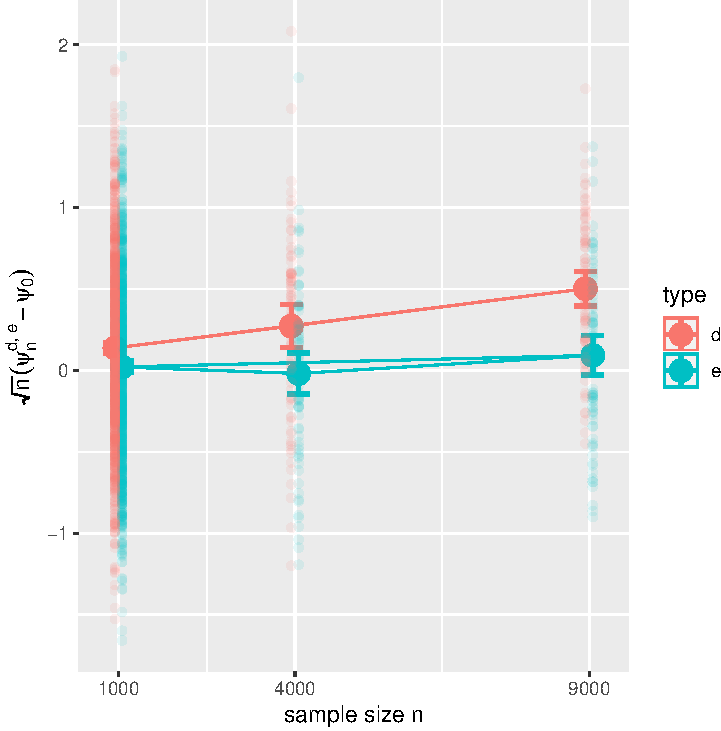
\includegraphics{img/estimating-Qbar-four-1.pdf}
\caption{\label{fig:estimating-Qbar-four}Evolution of root-\(n\) times bias
versus sample size for two inference methodology of \(\psi_{0}\) based
on the estimation of \(\Qbar_{0}\). Big dots represent the average
biases and vertical lines represent twice the standard error.}
\end{figure}

\subsection{One-step estimation.}
\label{subsec:one:step}

\subsection{Targeted inference.}
\label{subsec:tmle}

For later\(\ldots{}\)

\begin{Shaded}
\begin{Highlighting}[]
\NormalTok{working_model_Q_two <-}\StringTok{ }\KeywordTok{list}\NormalTok{(}
  \DataTypeTok{model =} \ControlFlowTok{function}\NormalTok{(...) \{}\KeywordTok{glm}\NormalTok{(}\DataTypeTok{family =} \KeywordTok{binomial}\NormalTok{(), ...)\},}
  \DataTypeTok{formula =} \KeywordTok{as.formula}\NormalTok{(}
    \KeywordTok{paste}\NormalTok{(}\StringTok{"Y ~ A * ("}\NormalTok{,}
          \KeywordTok{paste}\NormalTok{(}\StringTok{"I(W^"}\NormalTok{, }\KeywordTok{seq}\NormalTok{(}\DecValTok{1}\OperatorTok{/}\DecValTok{2}\NormalTok{, }\DecValTok{3}\NormalTok{, }\DataTypeTok{by =} \DecValTok{1}\OperatorTok{/}\DecValTok{2}\NormalTok{), }\DataTypeTok{sep =} \StringTok{""}\NormalTok{, }\DataTypeTok{collapse =} \StringTok{") + "}\NormalTok{),}
          \StringTok{"))"}\NormalTok{)}
\NormalTok{  ))}
\KeywordTok{attr}\NormalTok{(working_model_Q_two, }\StringTok{"ML"}\NormalTok{) <-}\StringTok{ }\OtherTok{FALSE}

\NormalTok{## xgboost based on trees}
\NormalTok{xgb_tree_algo <-}\StringTok{ }\ControlFlowTok{function}\NormalTok{(dat, ...) \{}
\NormalTok{  caret}\OperatorTok{::}\KeywordTok{train}\NormalTok{(Y }\OperatorTok{~}\StringTok{ }\KeywordTok{I}\NormalTok{(}\DecValTok{10}\OperatorTok{*}\NormalTok{A) }\OperatorTok{+}\StringTok{ }\NormalTok{W,}
               \DataTypeTok{data =}\NormalTok{ dat,}
               \DataTypeTok{method =} \StringTok{"xgbTree"}\NormalTok{,}
               \DataTypeTok{trControl =}\NormalTok{ control,}
               \DataTypeTok{tuneGrid =}\NormalTok{ grid,}
               \DataTypeTok{verbose =} \OtherTok{FALSE}\NormalTok{)  }
\NormalTok{\}}
\KeywordTok{attr}\NormalTok{(xgb_tree_algo, }\StringTok{"ML"}\NormalTok{) <-}\StringTok{ }\OtherTok{TRUE}
\NormalTok{xgb_tree_grid <-}\StringTok{ }\KeywordTok{expand.grid}\NormalTok{(}\DataTypeTok{nrounds =} \DecValTok{350}\NormalTok{,}
                             \DataTypeTok{max_depth =} \KeywordTok{c}\NormalTok{(}\DecValTok{4}\NormalTok{, }\DecValTok{6}\NormalTok{),}
                             \DataTypeTok{eta =} \KeywordTok{c}\NormalTok{(}\FloatTok{0.05}\NormalTok{, }\FloatTok{0.1}\NormalTok{),}
                             \DataTypeTok{gamma =} \FloatTok{0.01}\NormalTok{,}
                             \DataTypeTok{colsample_bytree =} \FloatTok{0.75}\NormalTok{,}
                             \DataTypeTok{subsample =} \FloatTok{0.5}\NormalTok{,}
                             \DataTypeTok{min_child_weight =} \DecValTok{0}\NormalTok{)}

\NormalTok{## nonparametric kernel smoothing regression}
\NormalTok{npreg <-}\StringTok{ }\KeywordTok{list}\NormalTok{(}
  \DataTypeTok{label =} \StringTok{"Kernel regression"}\NormalTok{,}
  \DataTypeTok{type =} \StringTok{"Regression"}\NormalTok{,}
  \DataTypeTok{library =} \StringTok{"np"}\NormalTok{,}
  \DataTypeTok{parameters =} \KeywordTok{data.frame}\NormalTok{(}\DataTypeTok{parameter =}
                            \KeywordTok{c}\NormalTok{(}\StringTok{"subsample"}\NormalTok{, }\StringTok{"regtype"}\NormalTok{,}
                              \StringTok{"ckertype"}\NormalTok{, }\StringTok{"ckerorder"}\NormalTok{), }
                          \DataTypeTok{class =} \KeywordTok{c}\NormalTok{(}\StringTok{"integer"}\NormalTok{, }\StringTok{"character"}\NormalTok{,}
                                    \StringTok{"character"}\NormalTok{, }\StringTok{"integer"}\NormalTok{), }
                          \DataTypeTok{label =} \KeywordTok{c}\NormalTok{(}\StringTok{"#subsample"}\NormalTok{, }\StringTok{"regtype"}\NormalTok{,}
                                    \StringTok{"ckertype"}\NormalTok{, }\StringTok{"ckerorder"}\NormalTok{)),}
  \DataTypeTok{grid =} \ControlFlowTok{function}\NormalTok{(x, y, }\DataTypeTok{len =} \OtherTok{NULL}\NormalTok{, }\DataTypeTok{search =} \StringTok{"grid"}\NormalTok{) \{}
    \ControlFlowTok{if}\NormalTok{ (}\OperatorTok{!}\KeywordTok{identical}\NormalTok{(search, }\StringTok{"grid"}\NormalTok{)) \{}
      \KeywordTok{stop}\NormalTok{(}\StringTok{"No random search implemented.}\CharTok{\textbackslash{}n}\StringTok{"}\NormalTok{)}
\NormalTok{    \} }\ControlFlowTok{else}\NormalTok{ \{}
\NormalTok{      out <-}\StringTok{ }\KeywordTok{expand.grid}\NormalTok{(}\DataTypeTok{subsample =} \KeywordTok{c}\NormalTok{(}\DecValTok{50}\NormalTok{, }\DecValTok{100}\NormalTok{),}
                         \DataTypeTok{regtype =} \KeywordTok{c}\NormalTok{(}\StringTok{"lc"}\NormalTok{, }\StringTok{"ll"}\NormalTok{),}
                         \DataTypeTok{ckertype =}
                           \KeywordTok{c}\NormalTok{(}\StringTok{"gaussian"}\NormalTok{,}
                             \StringTok{"epanechnikov"}\NormalTok{,}
                             \StringTok{"uniform"}\NormalTok{),}
                         \DataTypeTok{ckerorder =} \KeywordTok{seq}\NormalTok{(}\DecValTok{2}\NormalTok{, }\DecValTok{8}\NormalTok{, }\DecValTok{2}\NormalTok{))}
\NormalTok{    \} }
    \KeywordTok{return}\NormalTok{(out)}
\NormalTok{  \},}
  \DataTypeTok{fit =} \ControlFlowTok{function}\NormalTok{(x, y, wts, param, lev, last, classProbs, ...) \{}
\NormalTok{    ny <-}\StringTok{ }\KeywordTok{length}\NormalTok{(y)}
    \ControlFlowTok{if}\NormalTok{ (ny }\OperatorTok{>}\StringTok{ }\NormalTok{param}\OperatorTok{$}\NormalTok{subsample) \{}
\NormalTok{      ## otherwise far too slow for what we intend to do here...}
\NormalTok{      keep <-}\StringTok{ }\KeywordTok{sample.int}\NormalTok{(ny, param}\OperatorTok{$}\NormalTok{subsample)}
\NormalTok{      x <-}\StringTok{ }\NormalTok{x[keep, ]}
\NormalTok{      y <-}\StringTok{ }\NormalTok{y[keep]}
\NormalTok{    \}}
\NormalTok{    bw <-}\StringTok{ }\NormalTok{np}\OperatorTok{::}\KeywordTok{npregbw}\NormalTok{(}\DataTypeTok{xdat =} \KeywordTok{as.data.frame}\NormalTok{(x), }\DataTypeTok{ydat =}\NormalTok{ y,}
                      \DataTypeTok{regtype =}\NormalTok{ param}\OperatorTok{$}\NormalTok{regtype,}
                      \DataTypeTok{ckertype =}\NormalTok{ param}\OperatorTok{$}\NormalTok{ckertype,}
                      \DataTypeTok{ckerorder =}\NormalTok{ param}\OperatorTok{$}\NormalTok{ckerorder,}
                      \DataTypeTok{remin =} \OtherTok{FALSE}\NormalTok{, }\DataTypeTok{ftol =} \FloatTok{0.01}\NormalTok{, }\DataTypeTok{tol =} \FloatTok{0.01}\NormalTok{,}
\NormalTok{                      ...)}
\NormalTok{    np}\OperatorTok{::}\KeywordTok{npreg}\NormalTok{(bw)}
\NormalTok{  \},}
  \DataTypeTok{predict =} \ControlFlowTok{function}\NormalTok{ (modelFit, newdata, }\DataTypeTok{preProc =} \OtherTok{NULL}\NormalTok{, }\DataTypeTok{submodels =} \OtherTok{NULL}\NormalTok{) \{}
    \ControlFlowTok{if}\NormalTok{ (}\OperatorTok{!}\KeywordTok{is.data.frame}\NormalTok{(newdata)) \{}
\NormalTok{      newdata <-}\StringTok{ }\KeywordTok{as.data.frame}\NormalTok{(newdata)}
\NormalTok{    \}}
\NormalTok{    np}\OperatorTok{:::}\KeywordTok{predict.npregression}\NormalTok{(modelFit, }\DataTypeTok{se.fit =} \OtherTok{FALSE}\NormalTok{, newdata)}
\NormalTok{  \},}
  \DataTypeTok{sort =} \ControlFlowTok{function}\NormalTok{(x) \{}
\NormalTok{    x[}\KeywordTok{order}\NormalTok{(x}\OperatorTok{$}\NormalTok{regtype, x}\OperatorTok{$}\NormalTok{ckerorder), ]}
\NormalTok{  \},}
  \DataTypeTok{loop =} \OtherTok{NULL}\NormalTok{, }\DataTypeTok{prob =} \OtherTok{NULL}\NormalTok{, }\DataTypeTok{levels =} \OtherTok{NULL}
\NormalTok{)}

\NormalTok{npreg_algo <-}\StringTok{ }\ControlFlowTok{function}\NormalTok{(dat, ...) \{}
\NormalTok{  caret}\OperatorTok{::}\KeywordTok{train}\NormalTok{(working_model_Q_one}\OperatorTok{$}\NormalTok{formula,}
               \DataTypeTok{data =}\NormalTok{ dat,}
               \DataTypeTok{method =}\NormalTok{ npreg, }\CommentTok{# no quotes!}
               \DataTypeTok{verbose =} \OtherTok{FALSE}\NormalTok{,}
\NormalTok{               ...)}
\NormalTok{\}}
\KeywordTok{attr}\NormalTok{(npreg_algo, }\StringTok{"ML"}\NormalTok{) <-}\StringTok{ }\OtherTok{TRUE}
\NormalTok{npreg_grid <-}\StringTok{ }\KeywordTok{data.frame}\NormalTok{(}\DataTypeTok{subsample =} \DecValTok{100}\NormalTok{,}
                         \DataTypeTok{regtype =} \StringTok{"lc"}\NormalTok{,}
                         \DataTypeTok{ckertype =} \StringTok{"gaussian"}\NormalTok{,}
                         \DataTypeTok{ckerorder =} \DecValTok{4}\NormalTok{,}
                         \DataTypeTok{stringsAsFactors =} \OtherTok{FALSE}\NormalTok{)}
\end{Highlighting}
\end{Shaded}


\end{document}
